% \chapter{Equivariant ML for jets and anomaly detection}
% \label{sec:06_ml4jets}

% \chapter{Introduction}
% \label{sec:06_ml4jets_intro}

\ifdefined\HCode
    \chapter{Introduction and the JetNet Package}
\else
    \chapter{Introduction and the \jetnet Package}
\fi

\label{sec:06_jetnet}

In the final Part of the dissertation, we discuss some more developments in machine learning and high energy physics, focusing primarily on jets.
We first present the \jetnet Python package in Chapter~\ref{sec:06_jetnet}.
In the same spirit as the eponymous dataset introduced in Chapter~\ref{sec:04_intro}, it aims to increase the accessibility and reproducibility in our field by providing a standardized interface for accessing HEP datasets and benchmarking ML algorithms, as well as general utilities for ML and HEP.
Since its introduction in $2021$, it has become widely adopted by the community, with over 50,000 downloads, and has been used extensively for many exciting developments in the field, as described below.
By providing a common framework for jet datasets and evaluation metrics, it has also facilitated easy benchmarking and comparisons between different algorithms, particularly in the area of ML-based fast simulations, as discussed in Part~\ref{part:ml4sim}.

We then conclude this Part, and the dissertation, by presenting the first Lorentz-group-equivariant autoencoder (LGAE) in Chapter~\ref{sec:06_lgae}.
% We then have a brief interlude on the development, more generally, of \textit{equivariant} neural networks in Section~\ref{sec:06_equivariantnns}: ML models that are designed to respect intrinsic symmetries of the data, such as rotations, translations, and even Lorentz-boosts.
As detailed in Chapter~\ref{sec:03_ml_equivariantnns}, equivariant neural networks are extremely useful in the physical sciences, where data from sources such as molecules and high energy collisions naturally possess intrinsic physical symmetries, such as rotations, translations, and Lorentz-boosts.
Incorporating such \textit{inductive biases} of our data can lead to more data-efficient, interpretable, and performant AI algorithms.
Indeed, we find that the LGAE outperforms baseline, non-Lorentz-equivariant, models on tasks of compression and anomaly detection for jets, provides a more interpretable latent space, and achieves high performance with a small fraction of the data needed to train CNNs.

\ifdefined\HCode
    \section{JetNet}
\else
    \section{\texorpdfstring{\jetnet}{JetNet}}
\fi
\label{sec:06_jetnet_jetnet}

\begin{figure}[ht!]
    \centering
    \captionsetup{justification=centering}
    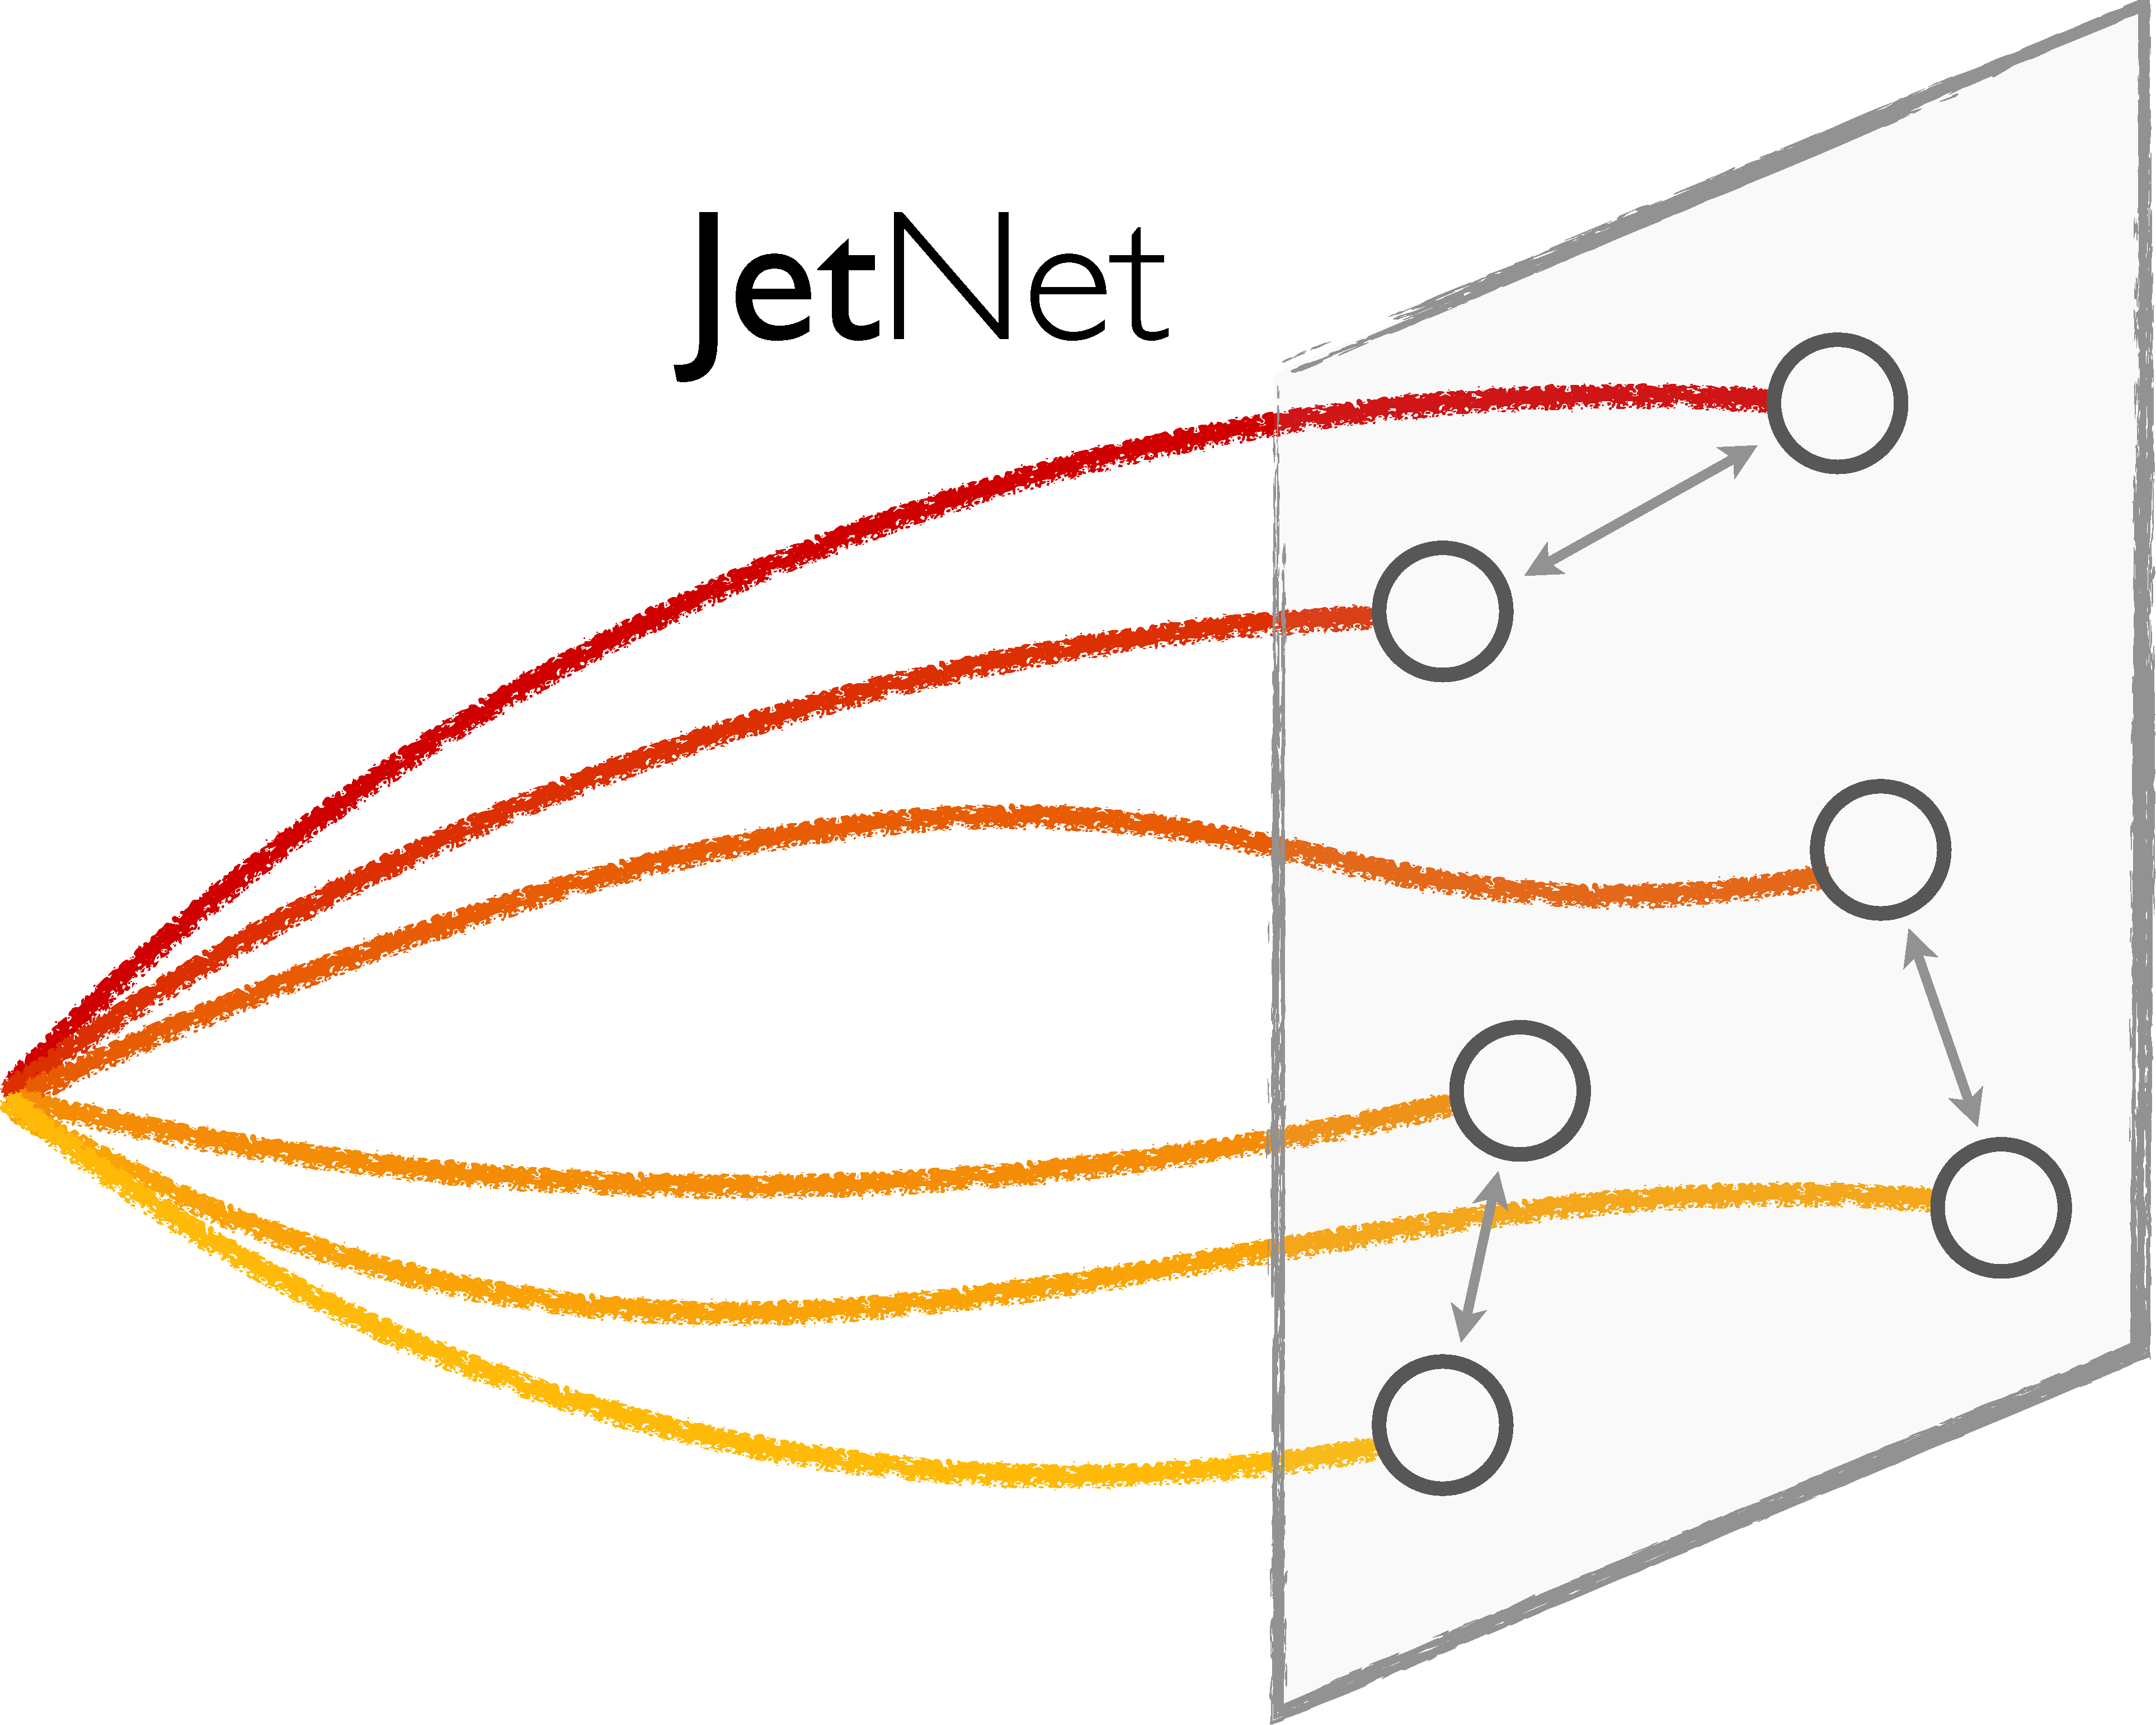
\includegraphics[width=0.5\textwidth]{figures/06-ML4Jets/jetnetlogo.pdf}
    \caption{The \jetnet logo.}
    \label{fig:06_jetnet_logo}
\end{figure}

% \jetnet is a Python package that aims to increase accessibility and reproducibility for ML in HEP, primarily focusing on jets.
% Based on the popular PyTorch ML framework, it provides easy-to-access and standardized interfaces for multiple heterogeneous HEP datasets and implementations of evaluation metrics, loss functions, and more general utilities relevant to HEP.

It is essential in scientific research to maintain standardized benchmark datasets following the findable, accessible, interoperable, and reproducible (FAIR) data principles~\cite{Chen:2021euv}, practices for using the data, and methods for evaluating and comparing different algorithms.
This can often be difficult in high energy physics (HEP) because of the broad set of formats in which data is released and the expert knowledge required to parse the relevant information.
The \jetnet Python package aims to facilitate this by providing a standard interface and format for HEP datasets, integrated with PyTorch~\cite{NEURIPS2019_9015}, to improve accessibility for both HEP experts and new or interdisciplinary researchers looking to do ML.
Furthermore, by providing standard formats and implementations for evaluation metrics, results are more easily reproducible, and models are more easily assessed and benchmarked.
\jetnet is complementary to existing efforts for improving HEP dataset accessibility, notably the \texttt{EnergyFlow} library~\cite{Komiske:2019jim}, with a unique focus to ML applications and integration with PyTorch.

\jetnet currently provides easy-to-access and standardized interfaces for the \jetnet dataset (Chapter~\ref{sec:04_jetnet_dataset}), top quark tagging~\cite{kasieczka_gregor_2019_2603256, Kasieczka:2019dbj}, and quark-gluon tagging~\cite{komiske_patrick_2019_3164691} reference datasets, all hosted on Zenodo~\cite{Zenodo}.
It also provides standard implementations of the generative evaluation metrics discussed in Chapter~\ref{sec:04_evaluating}, including Fr\'echet physics distance (FPD), kernel physics distance (KPD), 1-Wasserstein distance (W1), Fr\'echet ParticleNet distance (FPND), coverage, and minimum matching distance (MMD).
Finally, \jetnet implements as well custom loss functions like a differentiable version of the energy mover's distance~\cite{Komiske:2019fks} and more general jet utilities.
% \TODO{Can talk more about this? tie into learning EMD with the GNN too?}

\jetnet has had a considerable impact in the field, demonstrated by the surge in ML and HEP research it has facilitated, including in the areas of generative adversarial networks~\cite{Kansal:2021cqp}, transformers~\cite{Kach:2022uzq, Kansal:2022spb, Kach:2023rqw},  diffusion models~\cite{Leigh:2023toe, Mikuni:2023dvk}, and equivariant networks~\cite{Hao:2022zns, Buhmann:2023pmh}, all accessing datasets, metrics, and more through the package.
In particular, it has been the basis for virtually all research in the last two years on ML-based fast jet simulations~\cite{Kansal:2021cqp, Kach:2022uzq, Kansal:2022spb, Kach:2023rqw, Leigh:2023toe, Mikuni:2023dvk}, allowing objective comparisons and benchmarking of different algorithms; indeed, a planned direction for future work is a \jetnet community challenge collating all of these results.
We would also like to note that from the educational perspective, we have found \jetnet to be a valuable tool to involve new students quickly in ML research;
both through its use in easily initiating ML projects, as well as through contributions to the software itself.

In the future, we hope to expand the package to additional dataset loaders, including detector-level data, and different machine learning backends such as JAX~\cite{jax2018github}.
Improvements to the performance, such as optional lazy loading of large datasets, are also planned, as well as community challenges to benchmark algorithms as discussed above.

\subsubsection{Acknowledgements}

This chapter is, in part, a reprint of the materials as they appear in
JOSS, 2023, R. Kansal; C. Pareja; Z. Hao; and J. Duarte; JetNet: A Python package for accessing open datasets and benchmarking machine learning methods in high energy physics.
The dissertation author was the primary investigator and author of this paper.



\chapter{Lorentz-group equivariant autoencoders}
\label{sec:06_lgae}

\section{Introduction}
\label{sec:06_lgae_intro}

In this chapter, we present the first Lorentz-group-equivariant autoencoder (LGAE) for jets.
As described in Chapter~\ref{sec:03_genaes}, autoencoders are networks that learn to encode input data into, and decode data from, a low dimensional latent space, and thus have interesting applications in data compression~\cite{AE-data-compression-1,AE-data-compression-2} and anomaly detection~\cite{AE-anomaly,Atkinson:2021nlt,VAE-anomaly-VAE,Tsan:2021brw,Farina-anomaly,Finke-anomaly,VAE-anomaly-latent-space,QUAK}.
Both tasks are particularly relevant for HEP: the former to cope with the storage and processing of the ever-increasing data collected at the LHC; and the latter for model-agnostic searches for new physics.

Incorporating Lorentz equivariance into an autoencoder has the potential to not only increase performance in both respects, but also provide a more interpretable latent space and reduce training data requirements.
As discussed in Chapter~\ref{sec:03_ml_equivariantnns}, Lorentz symmetry has been successfully exploited recently in HEP for jet classification~\cite{bogatskiy2020lorentz,LorentzNet,Li:2022xfc,Butter_2018}, with competitive and even SOTA results.
In the same spirit, we aim to extend these developments to an autoencoder and explore its performance and interpretability.
To do so, we employ the Fourier space approach discussed above, which uses the set of irreducible representations (irreps) of the Lorentz-group as the basis for constructing equivariant maps.
We also train alternative architectures, including GNNs and convolutional neural networks (CNNs), with different inherent symmetries and find the LGAE outperforms them on reconstruction and anomaly detection tasks.

The principal results of this work demonstrate (1) that the advantage of incorporating Lorentz equivariance extends beyond whole jet classification to applications with particle-level outputs and (2) the interpretability of Lorentz-equivariant models.
The key challenges overcome in this work include: (1) training an equivariant autoencoder via particle-to-particle and permutation-invariant set-to-set losses (Section~\ref{sec:06_lgae_experiments}); (2) defining a jet-level compression scheme for the latent space (Section~\ref{sec:06_lgae_architecture}); and (3) optimizing the architecture for different tasks, such as reconstruction (Section~\ref{sec:06_lgae_reconstruction}) and anomaly detection (Section~\ref{sec:06_lgae_anomaly}).

This paper is structured as follows.
% In Section~\ref{sec:06_lgae_relatedwork}, we discuss existing work, motivating the LGAE.
We present the LGAE architecture in Section~\ref{sec:06_lgae_architecture}, and discuss experimental results on the reconstruction and anomaly detection of high energy jets in Section~\ref{sec:06_lgae_experiments}.
We also demonstrate the interpretability of the model, by analyzing its latent space, and its data efficiency relative to baseline models.
Finally, we conclude in Section~\ref{sec:06_lgae_conclusion}.


% \section{Related Work}
% \label{sec:06_lgae_relatedwork}

% In this section, we briefly recap progress in developing Lorentz-equivariant networks in Section~\ref{sec:06_lgae_lgenn} and applications of autoencoders in HEP in Section~\ref{sec:06_lgae_aehep}.

% \subsection{\label{sec:06_lgae_lgenn} Lorentz Group Equivariant Neural Networks}

% There have been some recent advances in incorporating this Lorentz-equivariance into NNs.
% As discussed in Section~\ref{sec:06_equivariantnns_lorentz}, the Lorentz group network (LGN)~\cite{bogatskiy2020lorentz} was the first such DNN, using an architecture similar to that of a GNN, but operating entirely in Fourier space on objects in irreps of the Lorentz group, and using tensor products between irreps and Clebsch--Gordan decompositions to introduce non-linearities in the network.
% More recently, LorentzNet~\cite{LorentzNet,Li:2022xfc} uses a similar GNN framework for equivariance, with additional edge features --- Minkowski inner products between node features --- but restricting itself to only scalar and vector representations of the group.
% Both networks have been successful in jet classification, with LorentzNet achieving SOTA results in top quark and quark versus gluon classification, further demonstrating the benefit of incorporating physical inductive biases into network architectures.
% In this work, we build on top of the LGN framework to go beyond outputting scalars alone (e.g. jet class probabilities) but encoding and reconstructing an input set of particles under the constraint of Lorentz group equivariance in an autoencoder-style architecture.




\section{LGAE architecture}
\label{sec:06_lgae_architecture}

\begin{figure}[htb!]
    \centering
    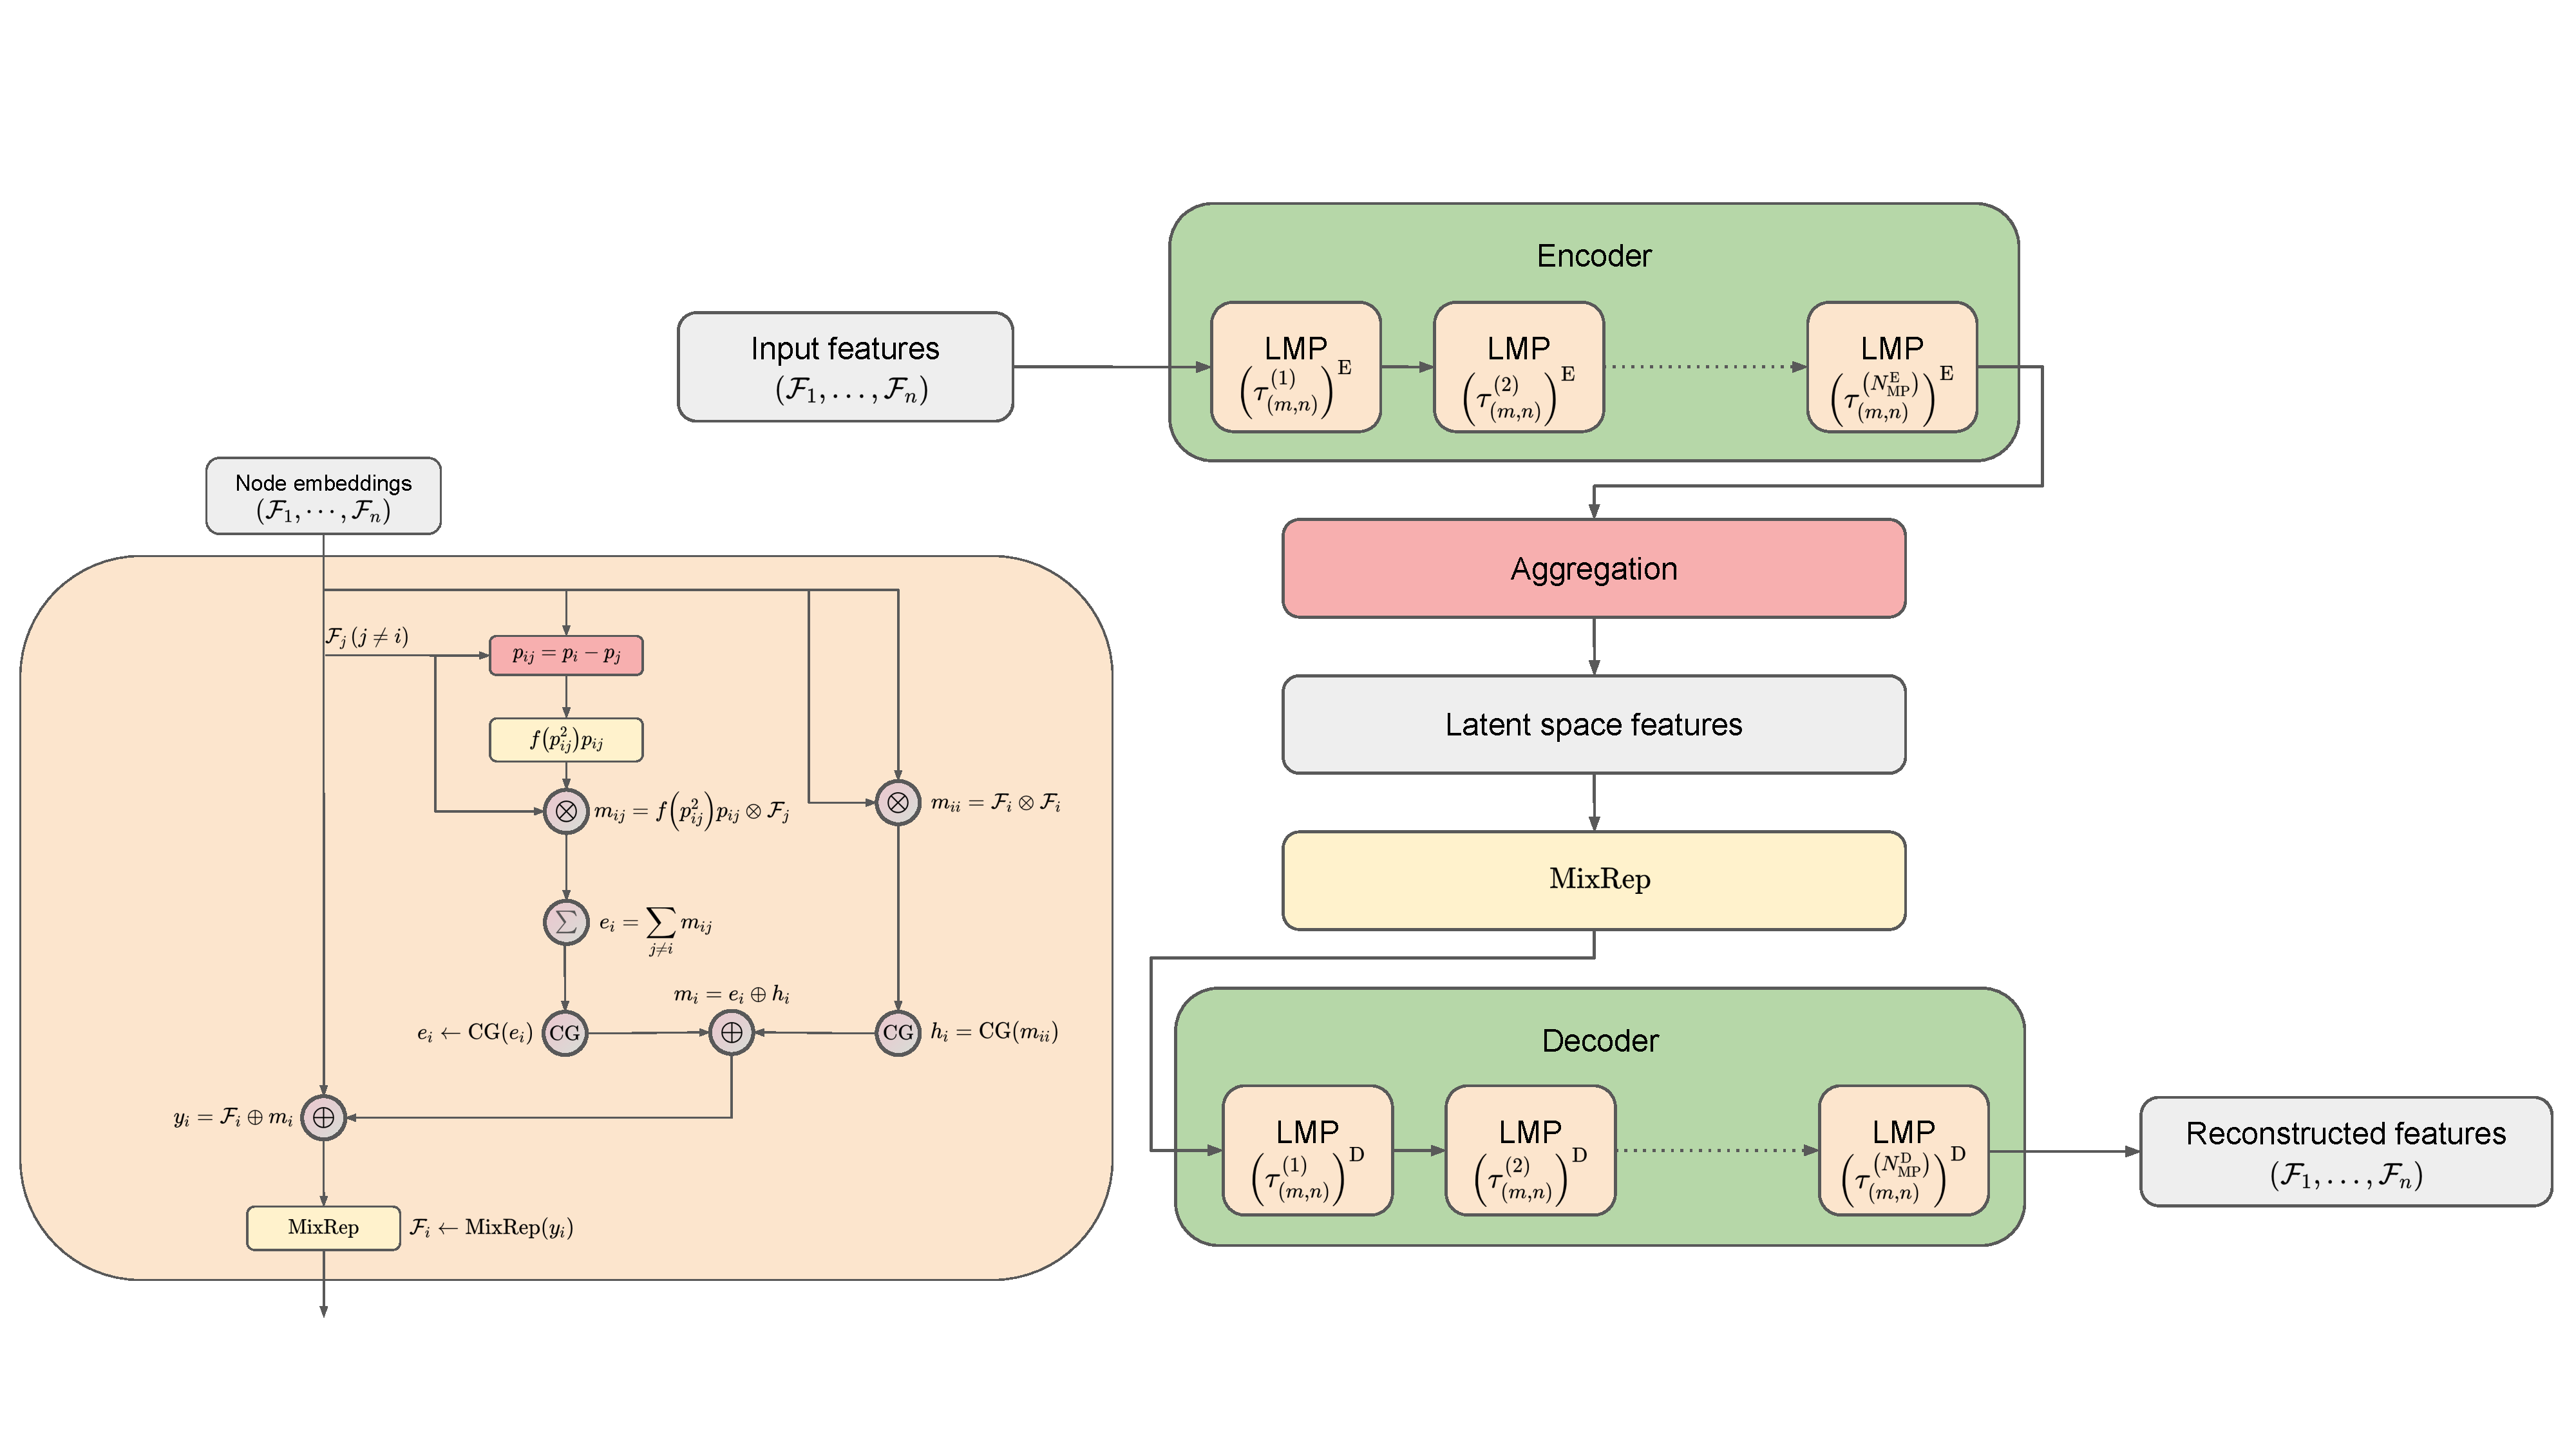
\includegraphics[width=\linewidth]{figures/06-ML4Jets/lgae/architectures/LGAE.pdf}
    \caption[Individual Lorentz group equivariant message passing (LMP) layers are shown on the left, and the LGAE architecture is built out of LMPs on the right.]{Individual Lorentz group equivariant message passing (LMP) layers are shown on the left, and the LGAE architecture is built out of LMPs on the right.
    Here, $\mathrm{MixRep}$ denotes the node-level operator that upsamples features in each $(m, n)$ representation space to $\tau_{(m, n)}$ channels; it appears as $W$ in Eq.~(\ref{eq:06_lgae_update}).}
    \label{fig:06_lgae_architecture-full}
\end{figure}


The LGAE is built out of Lorentz group-equivariant message passing (LMP) layers, which are identical to individual layers in the LGN~\cite{bogatskiy2020lorentz}.
We reinterpret them in the framework of message-passing neural networks~\cite{gilmer2017neural}, to highlight the connection to GNNs, and define them in Section~\ref{sec:06_lgae_lmp}.
We then describe the encoder and decoder networks in Sections~\ref{sec:06_lgae_lgaee} and \ref{sec:06_lgae_lgaed}, respectively.
The LMP layers and LGAE architecture are depicted in Figure~\ref{fig:06_lgae_architecture-full}.
We provide the LGAE code, written in Python using the \textsc{PyTorch} ML framework~\cite{pytorch} in Ref.~\cite{LGAE_code}.

\subsection{LMP layers \label{sec:06_lgae_lmp}}

LMP layers take as inputs fully-connected graphs with nodes representing particles and the Minkowski distance between respective node 4-vectors as edge features.
Each node $\mathcal{F}_i$ is defined by its features, all transforming under a corresponding irrep of the Lorentz group in the canonical basis~\cite{gelfand2018representations}, including at least one 4-vector (transforming under the $(1/2, 1/2)$ representation) representing its 4-momentum.
As in Ref~\cite{bogatskiy2020lorentz}, we denote the number of features in each node transforming under the $(m, n)$ irrep as $\tau_{(m,n)}$, referred to as the multiplicity of the $(m,n)$ representation.

The $(t+1)$-th MP layer operation consists of message-passing between each pair of nodes, with a message $m_{i j}^{(t)}$ to node $i$ from node $j$ (where $j \neq i$) and a self-interaction term $m_{ii}$ defined as
\begin{align} \label{eq:06_lgae_msg}
        m_{i j}^{(t)} &= f\left( \left(p_{ij}^{(t)}\right)^2 \right) p_{ij}^{(t)} \otimes \mathcal{F}_j^{(t)} \\
        m_{i i}^{(t)} &= \mathcal{F}_i^{(t)} \otimes \mathcal{F}_i^{(t)}
\end{align}
where $\mathcal{F}_{i}^{(t)}$ are the node features of node $i$ before the $(t+1)$-th layer, $p_{ij} = p_i - p_j$ is the difference between node four-vectors, $p_{ij}^2$ is the squared Minkowski norm of $p_{i j}$, and $f$ is a learnable, differentiable function acting on Lorentz scalars.
A Clebsch--Gordan (CG) decomposition, which reduces the features to direct sums of irreps of $\mathrm{SO}^+(3,1)$, is performed on both terms before concatenating them to produce the message $m_i$ for node $i$:
\begin{equation}
    m_i^{(t)} =
    \mathrm{CG}\left[
    m_{i i}^{(t)}
    \right]
    \oplus
    \mathrm{CG}\left[
    \sum_{j\neq i} m_{i j}^{(t)}
    \right],
\end{equation}
where the summation over the destination node $j$ ensures permutation symmetry because it treats all other nodes equally.

Finally, this aggregated message is used to update each node's features, such that
\begin{equation} \label{eq:06_lgae_update}
    \mathcal{F}_i^{(t+1)} = W^{(t+1)} \left( \mathcal{F}_i^{(t)} \oplus m_i^{(t)} \right)
\end{equation}
for all $i \in \{1, \ldots, N_{\mathrm{particle}}\}$, where $W^{(t+1)}$ is a learnable node-wise operator which acts as separate fully-connected linear layers $W^{(t+1)}_{(m, n)}$ on the set of components living within each separate $(m, n)$ representation space, outputting a chosen $\tau_{(m,n)}^{(t+1)}$ number of components per representation.
In practice, we then truncate the irreps to a maximum dimension to make computations more tractable.

\subsection{Encoder \label{sec:06_lgae_lgaee}}
The encoder takes as input an $N$-particle cloud, where each particle is each associated with a 4-momentum vector and an arbitrary number of scalars representing physical features such as mass, charge, and spin.
Each isotypic component is initially transformed to a chosen multiplicity of $\parenthesis{\tau_{(m, n)}^{(0)}}_{\mathrm{E}}$ via a node-wise operator $W^{(0)}$ identical conceptually to $W^{(t+1)}$ in Eq.~(\ref{eq:06_lgae_update}).
The resultant graph is then processed through $N_{\mathrm{MP}}^{\mathrm{E}}$ LMP layers, specified by a sequence of multiplicities $\left\{ \parenthesis{\tau_{(m, n)}^{(t)}}_{\mathrm{E}} \right\}_{t=1}^{N_{\mathrm{MP}}^{\mathrm{E}}}$, where $\parenthesis{\tau_{(m, n)}^{(t)}}_{\mathrm{E}}$ is the multiplicity of the $(m, n)$ representation at the $t$-th layer.
Weights are shared across the nodes in a layer to ensure permutation equivariance.
After the final MP layer, node features are aggregated to the latent space by a component-wise minimum (min), maximum (max), or mean.
The min and max operations are performed on the respective Lorentz invariants.
We also find, empirically, interesting performance by simply concatenating isotypic components across each particle and linearly ``mixing" them via a learned matrix as in Eq.~(\ref{eq:06_lgae_update}).
Crucially, unlike in Eq.~(\ref{eq:06_lgae_update}), where this operation only happens per particle, the concatenation across the particles imposes an ordering and, hence, breaks the permutation symmetry.


\subsection{Decoder \label{sec:06_lgae_lgaed}}

The decoder recovers the $N$-particle cloud by acting on the latent space with $N$ independent, learned linear operators, which again mix components living in the same representations.
This cloud passes through $N_{\mathrm{MP}}^{\mathrm{D}}$ LMP layers, specified by a sequence of multiplicities $\left\{ \parenthesis{\tau_{(m, n)}^{(t)}}_{\mathrm{D}} \right\}_{t=1}^{N_{\mathrm{MP}}^{\mathrm{D}}}$, where $\parenthesis{\tau_{(m, n)}^{(t)}}_{\mathrm{D}}$ is the multiplicity of the $(m, n)$ representation at the $t$-th LMP layer.
After the LMP layers, node features are mixed back to the input representation space $\parenthesis{D^{(0,0)}}^{\oplus \tau_{(0,0)}^{(0)}} \oplus D^{(1/2, 1/2)}$ by applying a linear mixing layer and then truncating other isotypic components.

\section{Experiments}
\label{sec:06_lgae_experiments}

We experiment with and evaluate the performance of the LGAE and baseline models on reconstruction and anomaly detection for simulated high-momentum jets from the \jetnet dataset.
In this section, we describe the dataset in more detail in Section~\ref{sec:06_lgae_dataset}, the different models we consider in Section~\ref{sec:06_lgae_models}, the reconstruction and anomaly detection results in Sections~\ref{sec:06_lgae_reconstruction} and~\ref{sec:06_lgae_anomaly} respectively, an interpretation of the LGAE latent space in Section~\ref{sec:06_lgae_latent-analysis}, and finally experiments of the data efficiency of the different models in Section~\ref{sec:06_lgae_data-efficiency}.

\subsection{Dataset}
\label{sec:06_lgae_dataset}

We use 30-particle high \pt jets from the \jetnet dataset as described in Chapter~\ref{sec:04_jetnet_dataset}, obtained using the \jetnet library from Chapter~\ref{sec:06_jetnet}.
The model is trained on jets produced from gluons and light quarks, which are collectively referred to as quantum chromodynamics (QCD) jets.

As before, we represent the jets as a point cloud of particles, termed a ``particle cloud'', with the respective 3-momenta, in absolute coordinates, as particle features.
In the processing step, each 3-momentum is converted to a 4-momentum: $p^\mu = (|\mathbf{p}|, \mathbf{p})$, where we consider the mass of each particle to be negligible.
We use a $60\%/20\%/20\%$ training/testing/validation splitting for the total 177,000 jets.
For evaluating performance in anomaly detection, we consider jets from \jetnet produced by top quarks, $W$ bosons, and $Z$ bosons as our anomalous signals.

We note that the detector and reconstruction effects in \jetnet, and indeed in real data collected at the LHC, break the Lorentz symmetry; hence, Lorentz equivariance is generally an \textit{approximate} rather than an exact symmetry of HEP data.
We assume henceforth that the magnitude of the symmetry breaking is small enough that imposing exact Lorentz equivariance in the LGAE is still advantageous --- and the high performance of the LGAE and classification models such as LorentzNet support this assumption.
Nevertheless, important studies in future work may include quantifying this symmetry breaking and considering approximate symmetries in NNs.

\subsection{Models}
\label{sec:06_lgae_models}

LGAE model results are presented using both the min-max (LGAE-Min-Max) and ``mix'' (LGAE-Mix) aggregation schemes for the latent space, which consists of varying numbers of complex Lorentz vectors --- corresponding to different compression rates.
We compare the LGAE to baseline GNN and CNN autoencoder models, referred to as ``GNNAE'' and ``CNNAE'' respectively.

The GNNAE model is composed of fully-connected MPNNs adapted from MPGAN (Section~\ref{sec:04_mpgan}).
We experiment with two types of encodings: (1) particle-level (GNNAE-PL), as in the PGAE~\cite{Tsan:2021brw} model, which compresses the features per node in the graph but retains the graph structure in the latent space, and (2) jet-level (GNNAE-JL), which averages the features across each node to form the latent space, as in the LGAE.
Particle-level encodings produce better performance overall for the GNNAE, but the jet-level provides a more fair comparison with the LGAE, which uses jet-level encoding to achieve a high level of compression of the features.

For the CNNAE, which is adapted from Ref.~\cite{Farina-anomaly}, the relative coordinates of each input jets' particle constituents are first discretized into a $40 \times 40$ grid.
The particles are then represented as pixels in an image, with intensities corresponding to $\ptrel$.
Multiple particles per jet may correspond to the same pixel, in which case their \ptrel's are summed.
The CNNAE has neither Lorentz nor permutation symmetry, however, it does have in-built translation equivariance in $\eta-\phi$ space.

Hyperparameter and training details for all models can be found in~\ref{app:06_lgae_hyperparams} and~\ref{app:06_lgae_training}, respectively, and a summary of the relevant symmetries respected by each model is provided in Table~\ref{tab:06_lgae_model-symmetry}.
The LGAE models are verified to be equivariant to Lorentz boosts and rotations up to numerical error, with details provided in~\ref{app:06_lgae_equivariancetests}.

\begin{table}[t!]
    \centering
    \captionsetup{justification=centering}
    \caption{Summary of the relevant symmetries respected by each model tested.}
    \label{tab:06_lgae_model-symmetry}
    \resizebox{\textwidth}{!}{
    \begin{tabular}{llllll}
        \toprule
        Model                  & Aggregation    & Name                    & Lorentz symmetry        & Permutation symmetry  & Translation symmetry  \\ \midrule
        \multirow{2}{*}{LGAE}  &
        Min-Max                & LGAE-Min-Max   & \checkmark (equivariance) & \checkmark (invariance)  & \checkmark (equivariance)                           \\
                               & Mix            & LGAE-Mix                & \checkmark (equivariance) & \xmark   & \checkmark (equivariance)               \\[2mm]
        \multirow{2}{*}{GNNAE} &
        Jet-level              & GNNAE-JL       & \xmark                  & \checkmark (invariance) & \checkmark (equivariance)                          \\
                               & Particle-level & GNNAE-PL                & \xmark                  & \checkmark (equivariance) & \checkmark (equivariance) \\[2mm]
        CNNAE & & CNNAE & \xmark  & \xmark & \checkmark (equivariance) \\
        \cbottomrule
    \end{tabular}
    }
\end{table}

\subsection{Reconstruction}
\label{sec:06_lgae_reconstruction}

\begin{figure}[ht!]
    \centering
    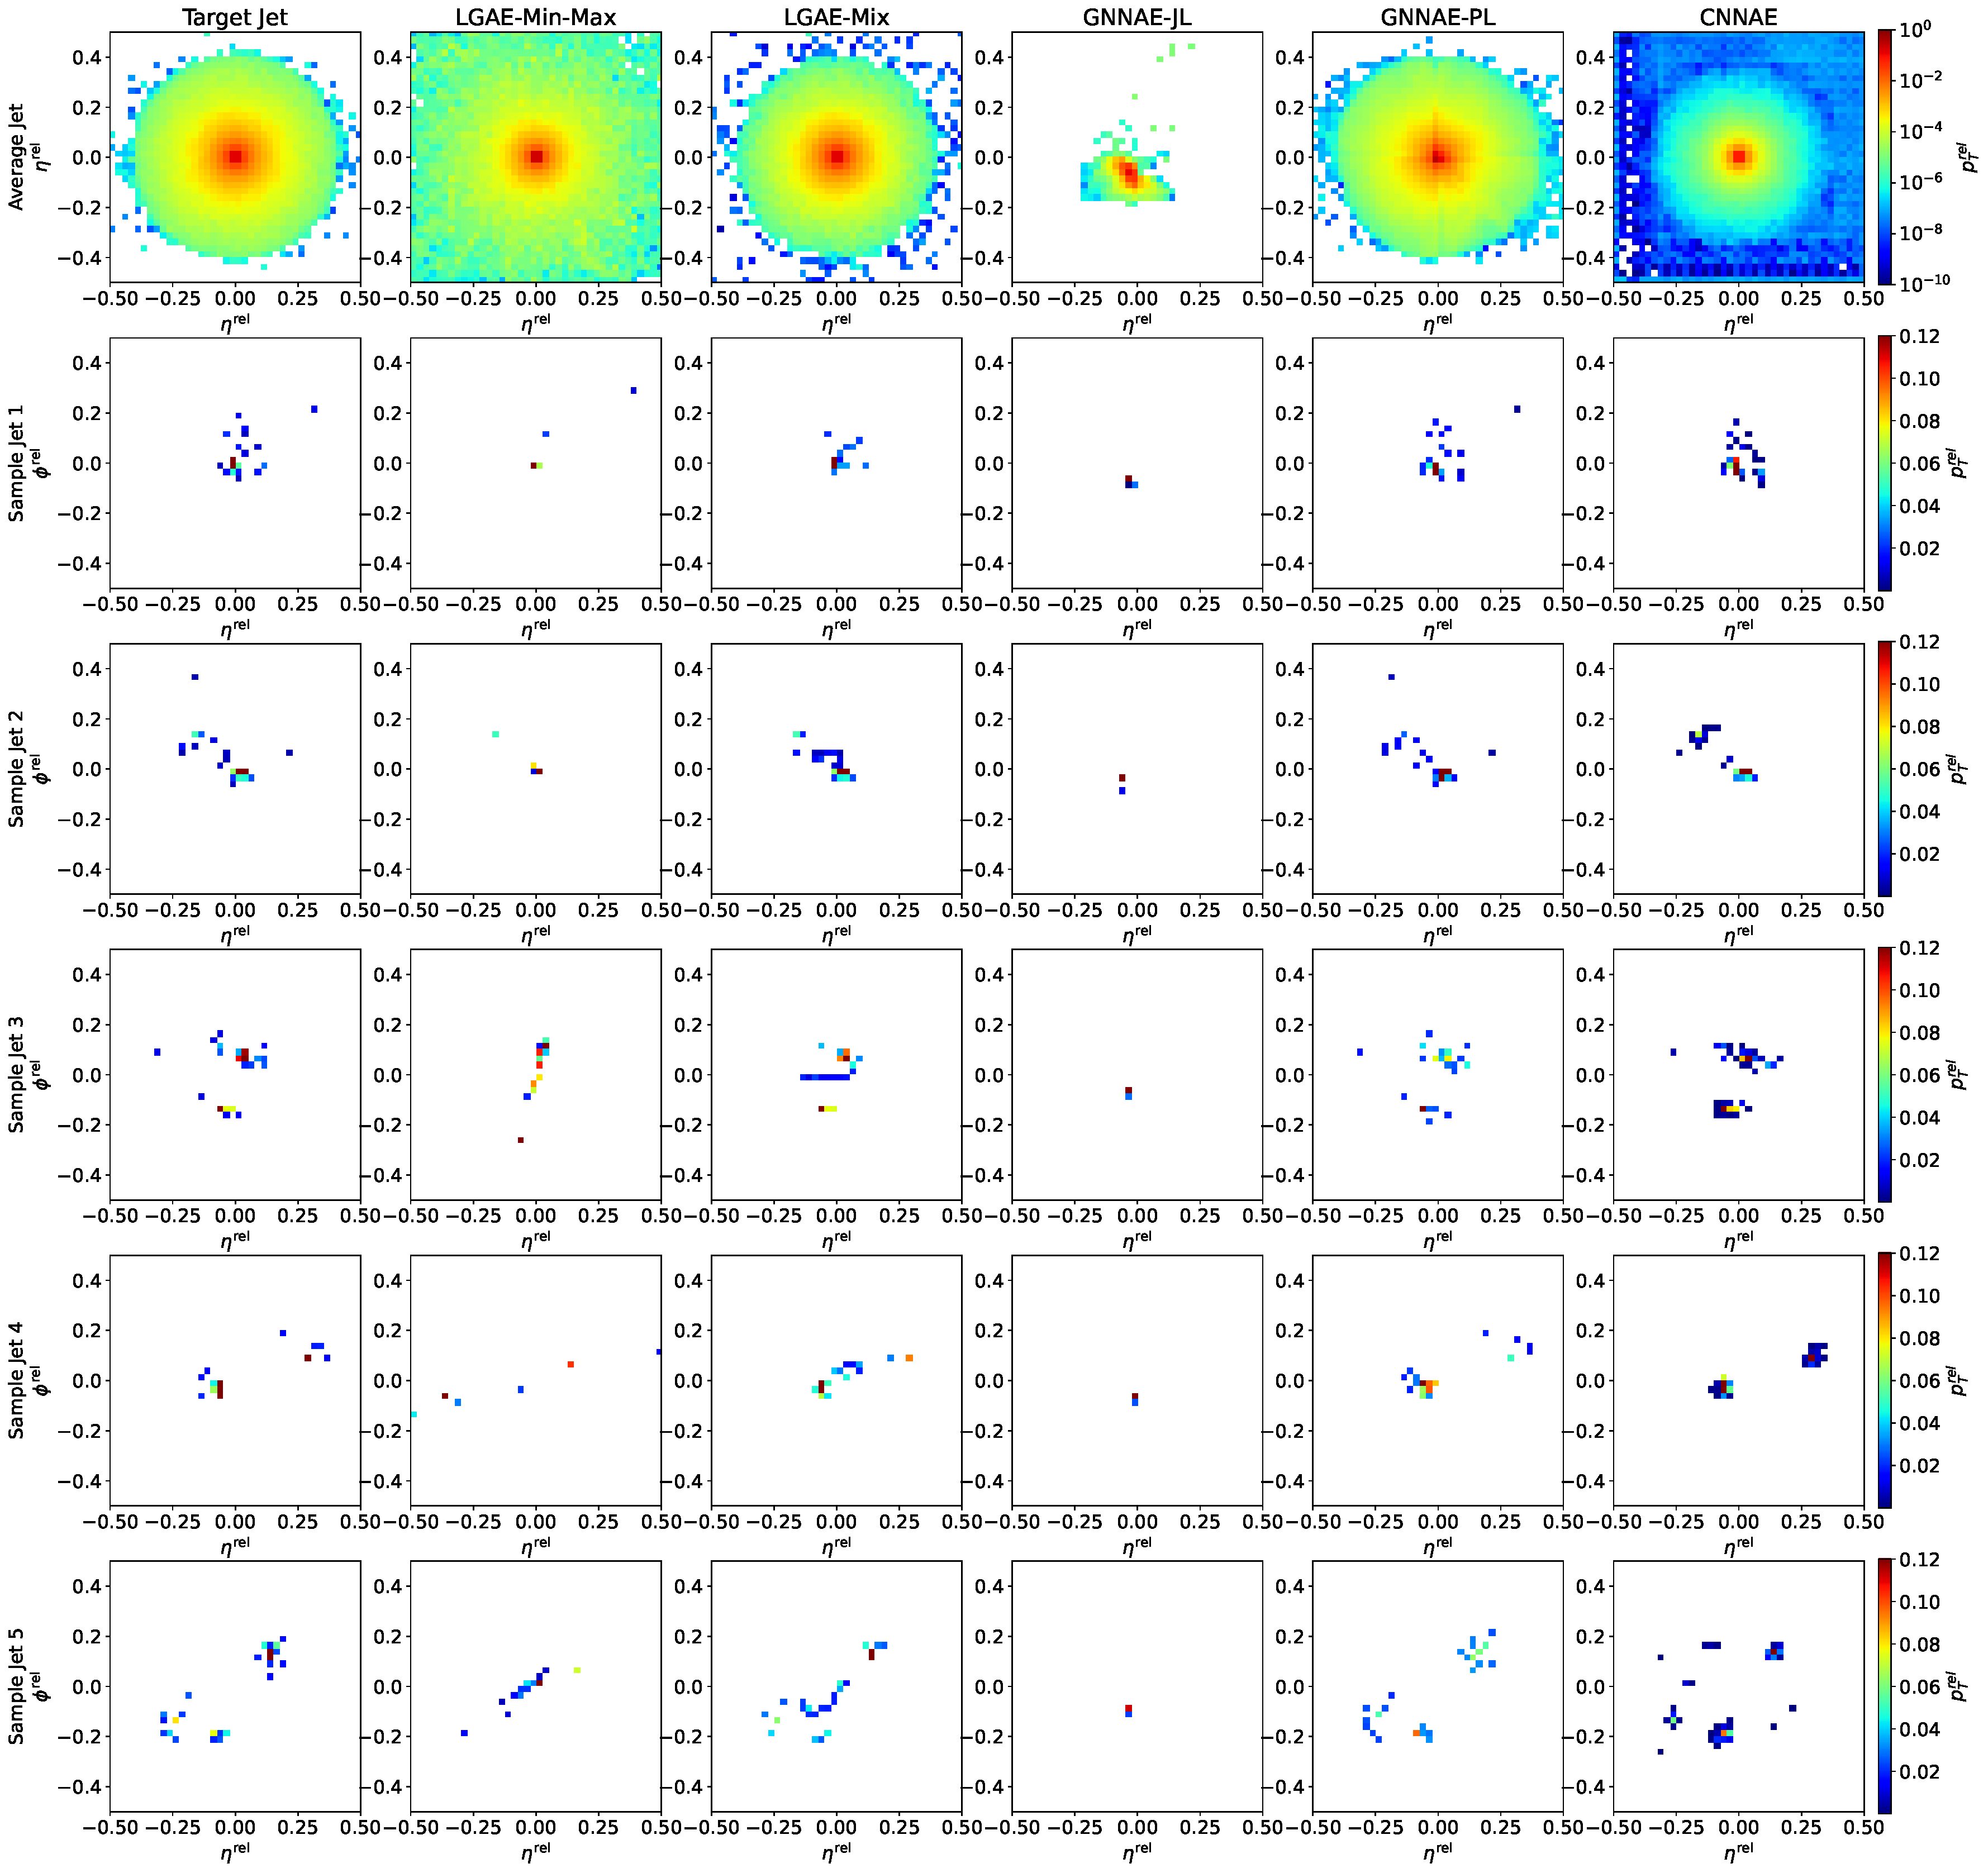
\includegraphics[width=\linewidth]{figures/06-ML4Jets/lgae/reconstructions/jet_images-cnnae.pdf}
    \caption[Jet image reconstructions.]{Jet image reconstructions by
        LGAE-Min-Max ($\tau_{(1/2, 1/2)}=4$, $56.67\%$ compression),
        LGAE-Mix ($\tau_{(1/2, 1/2)}=9$, $61.67\%$ compression),
        GNNAE-JL ($\dim(L) = 55$, $61.11\%$ compression),
        GNNAE-PL ($\dim(L) = 2\times 30$, $66.67\%$ compression), and CNNAE ($\dim(L) = 55$, $61.11\%$ compression).
    }
    \label{fig:06_lgae_recons-jet-imgs}
\end{figure}


We evaluate the performance of the LGAE, GNNAE, and CNNAE models, with the different aggregation schemes discussed, on the reconstruction of the particle and jet features of QCD jets.
We consider relative transverse momentum
$\ptrel = p_{\mathrm{T}}^{\mathrm{particle}}/p_{\mathrm{T}}^{\mathrm{jet}}$ and relative angular coordinates
$\etarel =\eta^{\mathrm{particle}} - \eta^{\mathrm{jet}}$ and
$\phirel =\phi^{\mathrm{particle}} - \phi^{\mathrm{jet}} \pmod{2\pi}$
as each particle's features, and total jet mass, \pt and $\eta$ as jet features.
We define the compression rate as the ratio between the total dimension of the latent space and the number of features in the input space: $30\ \mathrm{particles} \times 3\ \mathrm{features\ per\ particle} = 90$.

Figure~\ref{fig:06_lgae_recons-jet-imgs} shows random samples of jets, represented as discrete images in the angular-coordinate plane, reconstructed by the models with similar levels of compression in comparison to the true jets.
Figure~\ref{fig:06_lgae_recons-hist} shows histograms of the reconstructed features compared to the true distributions.
The differences between the two distributions are quantified in Table~\ref{tab:06_lgae_recons-particle} by calculating the median and interquartile ranges (IQR) of the relative errors between the reconstructed and true features.
To calculate the relative errors of particle features for the permutation invariant LGAE and GNNAE models, particles are matched between the input and output clouds using the Jonker–Volgenant algorithm~\cite{JonkerVolgenant,2020SciPy-NMeth} based on the L2 distance between particle features.
Due to the discretization of the inputs to the CNNAE, reconstructing individual particle features is not possible; instead, only jet features are shown.\footnote{These are calculated by summing each pixel's momentum ``4-vector'' --- using the center of the pixel as angular coordinates and intensity as the \ptrel.}

We can observe visually in Figure~\ref{fig:06_lgae_recons-jet-imgs} that out of the two permutation invariant models, while neither is able to reconstruct the jet substructure perfectly,
the LGAE-Min-Max outperforms the GNNAE-JL.
Perhaps surprisingly, the permutation-symmetry-breaking mix aggregation scheme improves the LGAE in this regard.
Both visually in Figure~\ref{fig:06_lgae_recons-hist} and quantitatively from Tables~\ref{tab:06_lgae_recons-particle} and~\ref{tab:06_lgae_recons-jet}, we conclude that the LGAE-Mix has the best performance overall, significantly outperforming the GNNAE and CNNAE models at similar compression rates.
The LGAE-Min-Max model outperforms the GNNAE-JL in reconstructing all features and the GNNAE-PL in all but the IQR of the particle angular coordinates.

\begin{figure}[ht!]
    \centering
    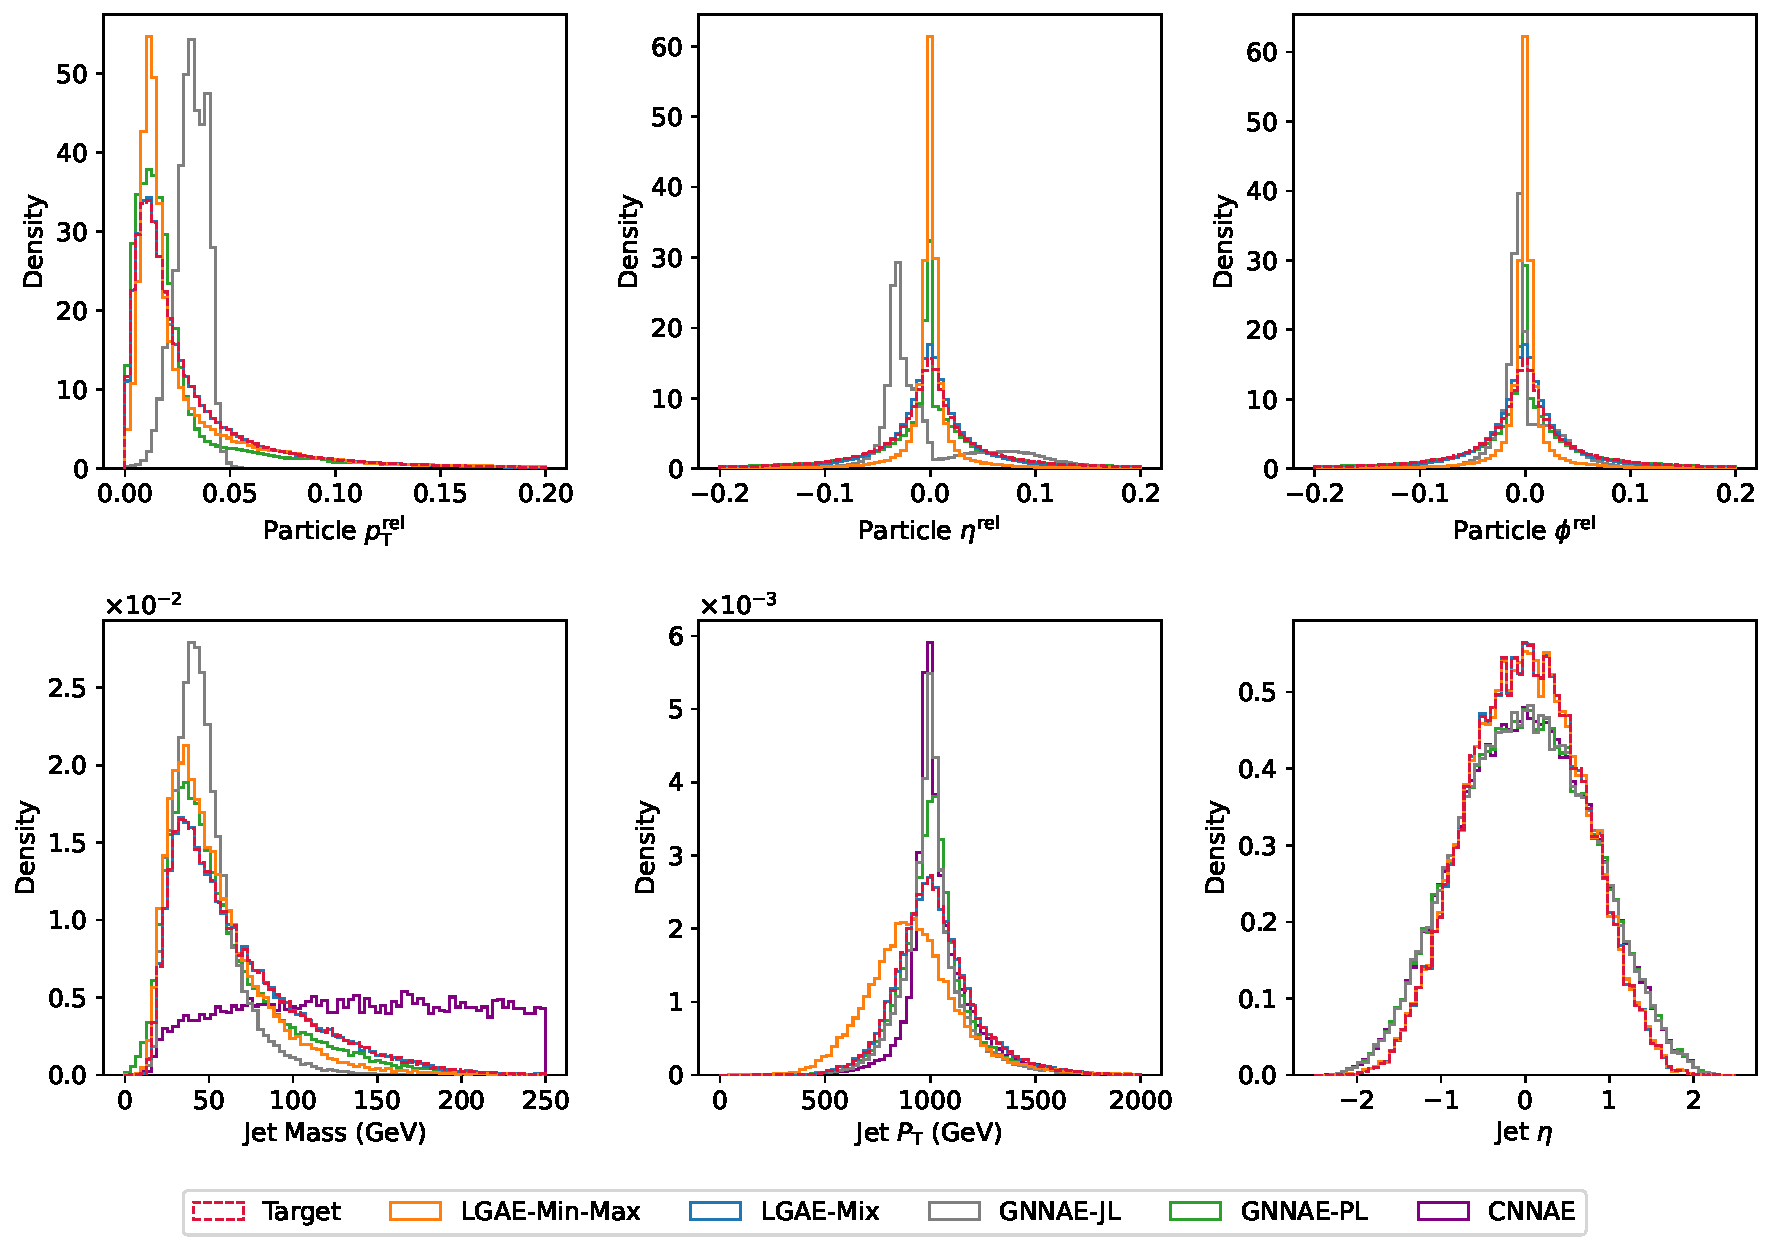
\includegraphics[width=\linewidth]{figures/06-ML4Jets/lgae/reconstructions/hist-cnnae.pdf}
    \caption[Particle and jet feature reconstruction by the LGAE, GNNAE, and CNNAE models.]{
        \textbf{Top}:
        particle momenta $(\ptrel, \eta^{\mathrm{rel}}, \phi^{\mathrm{rel}})$ reconstruction by
        LGAE-Min-Max ($\tau_{(1/2, 1/2)}=4$, resulting in $56.67\%$ compression) and
        and LGAE-Mix ($\tau_{(1/2, 1/2)}=9$, resulting in $61.67\%$ compression),
        and GNNAE-JL ($\dim(L) = 55$, resulting in $61.11\%$ compression) and
        GNNAE-PL ($\dim(L) = 2\times 30$, resulting in $66.67\%$ compression). The reconstructions by the CNNAE are not included due to the discrete values of $\etarel$ and $\phirel$, as discussed in the text.
        \textbf{Bottom}:
        jet feature $(M, \pt, \eta)$ reconstruction by the four models.
        For the jet feature reconstruction by the GNNAEs, the particle features in relative coordinates were transformed back to absolute coordinates before plotting.
        The jet $\phi$ is not shown because it follows a uniform distribution in $(-\pi, \pi]$ and is reconstructed well.
    }
    \label{fig:06_lgae_recons-hist}
\end{figure}

\begin{table}[ht!]
    \centering
    \caption{Median and IQR of relative errors in particle feature reconstruction of selected LGAE and GNNAE models.
        In each column, the best-performing latent space per model is italicized, and the best model overall is highlighted in bold.
    }
    \label{tab:06_lgae_recons-particle}
    \resizebox{\textwidth}{!}{
    \begin{tabular}{lllcccccc }  \toprule
        \multirow{2}{*}{Model}
        & \multirow{2}{*}{Aggregation}
        & \multirow{2}{*}{Latent space}
        & \multicolumn{2}{c}{Particle \ptrel}
        & \multicolumn{2}{c}{Particle \etarel}
        & \multicolumn{2}{c}{Particle \phirel}
        \\ \cline{4-9}
        &&& Median & IQR & Median & IQR & Median & IQR
        \\ \midrule
        \multirow{4}{*}{LGAE} & \multirow{2}{*}{Min-max}
        & $\tau_{(1/2, 1/2)} = 4$ ($56.67\%$)
        & $\mathit{0.006}$ & $\mathit{0.562}$
        & $\mathit{0.002}$ & ${1.8}$
        & ${0.003}$ & ${1.8}$                              \\ &
        & $\tau_{(1/2, 1/2)} = 7$ ($96.67\%$)
        & $0.002$ & $0.640$
        & $-0.627$ & $\mathit{1.7}$
        & $\mathbf{< 10^{-3}}$ & $\mathit{1.7}$                       \\[1mm]
        & \multirow{2}{*}{Mix}
        & $\tau_{(1/2, 1/2)} = 9$ ($61.67\%$)
        & $\mathbf{< 10^{-3}}$ & $0.011$
        & $\mathbf{< 10^{-3}}$ & $0.452$
        & $\mathbf{< 10^{-3}}$ & ${0.451}$
        \\
        & & $\tau_{(1/2, 1/2)} = 13$ ($88.33\%$)
        & $\mathbf{< 10^{-3}}$ & $\mathbf{0.001}$
        & $\mathbf{< 10^{-3}}$ & $\mathbf{0.022}$
        & $\mathbf{< 10^{-3}}$ & $\mathbf{0.022}$                     \\[2mm]
        \multirow{4}{*}{GNNAE}
    & \multirow{2}{*}{Jet-level}
    & $\dim(L) = 45$ ($50.00\%$)
    & $-0.983$ & $3.8$
    & $\mathit{0.363}$ & $\mathit{3.1}$
    & $\mathit{0.146}$ & $\mathit{2.1}$                       \\
    & & $\dim(L) = 90$ ($100.00\%$)
    & $\mathit{-0.627}$ & $\mathit{3.5}$
    & $4.4$ & ${14.7}$
    & $\mathit{0.146}$ & ${2.6}$                              \\[1mm]
    & \multirow{2}{*}{Particle-level}
    & $\dim(L) = 2 \times 30$ ($66.67\%$)
    & $-0.053$ & $0.906$
    & $\mathit{0.009}$ & ${0.191}$
    & ${0.013}$ & $\mathit{0.139}$                     \\
    & & $\dim(L) = 3 \times 30$ ($100.00\%$)
    & $\mathit{-0.040}$ & $\mathit{0.892}$
    & ${-0.037}$ & $\mathit{0.177}$
    & $\mathit{0.005}$ & $0.243$                              \\
        \cbottomrule
    \end{tabular}
    }
\end{table}



\begin{table}[ht!]
    \centering
    \caption[Median and IQR of relative errors in jet feature
    reconstruction by selected LGAE and GNNAE models, along with the CNNAE model.]{Median and IQR of relative errors in jet feature
        reconstruction by selected LGAE and GNNAE models, along with the CNNAE model.
        In each column, the best performing latent space per model is italicised, and the best model overall is highlighted in bold.
    }
    \label{tab:06_lgae_recons-jet}
    \resizebox{\textwidth}{!}{
    \begin{tabular}{lllcccccccc}  \toprule
        \multirow{2}{*}{Model}
         & \multirow{2}{*}{Aggregation}
         & \multirow{2}{*}{Latent space}
         & \multicolumn{2}{c}{Jet mass}
         & \multicolumn{2}{c}{Jet $\pt$}
         & \multicolumn{2}{c}{Jet $\eta$}
         & \multicolumn{2}{c}{Jet $\phi$}
        \\ \cline{4-11}
         & &
         & Median & IQR
         & Median & IQR
         & Median & IQR
         & Median & IQR
        \\ \midrule
        \multirow{4}{*}{LGAE}
         & \multirow{2}{*}{Min-max}
         & $\tau_{(1/2,1/2)} = 4$ ($56.67\%$)
         & $\mathit{0.096}$ & $\mathit{0.134}$
         & $\mathit{0.097}$ & $\mathit{0.109}$
         & $\mathbf{< 10^{-3}}$ & $\mathit{0.004}$
         & $\mathbf{< 10^{-3}}$ & $\mathit{0.002}$
        \\
         & & $\tau_{(1/2,1/2)} = 7$ ($96.67\%$)
         & ${-0.139}$ & ${0.287}$
         & ${-0.221}$ & ${0.609}$
         & $\mathbf{< 10^{-3}}$ & ${0.021}$
         & $\mathbf{< 10^{-3}}$ & ${0.007}$
        \\[1mm]
         & \multirow{2}{*}{Mix}
         & $\tau_{(1/2,1/2)} = 9$ ($61.67\%$)
         & $\mathbf{< 10^{-3}}$ & $\mathbf{0.003}$
         & $\mathbf{< 10^{-3}}$ & $\mathbf{< 10^{-3}}$
         & $\mathbf{< 10^{-3}}$
         & $\mathbf{< 10^{-3}}$
         & $\mathbf{< 10^{-3}}$ &
         $\mathbf{< 10^{-3}}$
        \\
         & & $\tau_{(1/2,1/2)} = 13$ ($88.33\%$)
         & $\mathbf{< 10^{-3}}$ & $\mathbf{0.003}$
         & $\mathbf{< 10^{-3}}$ & $\mathbf{< 10^{-3}}$
         & $\mathbf{< 10^{-3}}$
         & $\mathbf{< 10^{-3}}$
         & $\mathbf{< 10^{-3}}$ &
         $\mathbf{< 10^{-3}}$
        \\[2mm]
        \multirow{4}{*}{GNNAE}
         & \multirow{2}{*}{Jet-level}
         & $\dim(L) = 45$ ($50.00\%$)
         & ${0.326}$ & $\mathit{0.667}$
         & $\mathit{0.030}$ & $\mathit{0.088}$
         & $\mathit{0.005}$ & $\mathit{0.040}$
         & $\mathit{0.001}$ & ${0.021}$
        \\
         & & $\dim(L) = 90$ ($100.00\%$)
         & ${3.7}$ & $2.6$
         & $\mathit{0.030}$ & ${0.089}$
         & ${0.292}$ & ${0.433}$
         & ${0.006}$ & ${0.021}$
        \\[1mm]
         & \multirow{2}{*}{Particle-level}
         & $\dim(L) = 2 \times 30$ ($66.67\%$)
         & $\mathit{0.277}$ & ${0.299}$
         & $\mathit{0.037}$ & ${0.110}$
         & ${0.002}$ & $\mathit{0.010}$
         & $-0.001$ & ${0.005}$
        \\
         & & $\dim(L) = 3 \times 30$ ($100.00\%$)
         & ${0.339}$ & $\mathit{0.244}$
         & ${0.050}$ & $\mathit{0.094}$
         & $\mathit{-0.001}$ & ${0.011}$
         & $\mathbf{<10^{-3}}$ & ${0.005}$
        \\[2mm]
        CNNAE
        & Linear layer
        & $\dim(L) = 55$ ($61.67\%$)
        & $-0.030$
        & $0.042$
        & $-0.021$
        & $0.017$
        & $\mathbf{< 10^{-3}}$
        & $0.017$
        & $\mathbf{<10^{-3}}$
        & $0.003$ \\
        \cbottomrule
    \end{tabular}
    }
\end{table}

\clearpage
\subsection{Anomaly detection}
\label{sec:06_lgae_anomaly}

\begin{figure}[ht!]
    \centering
    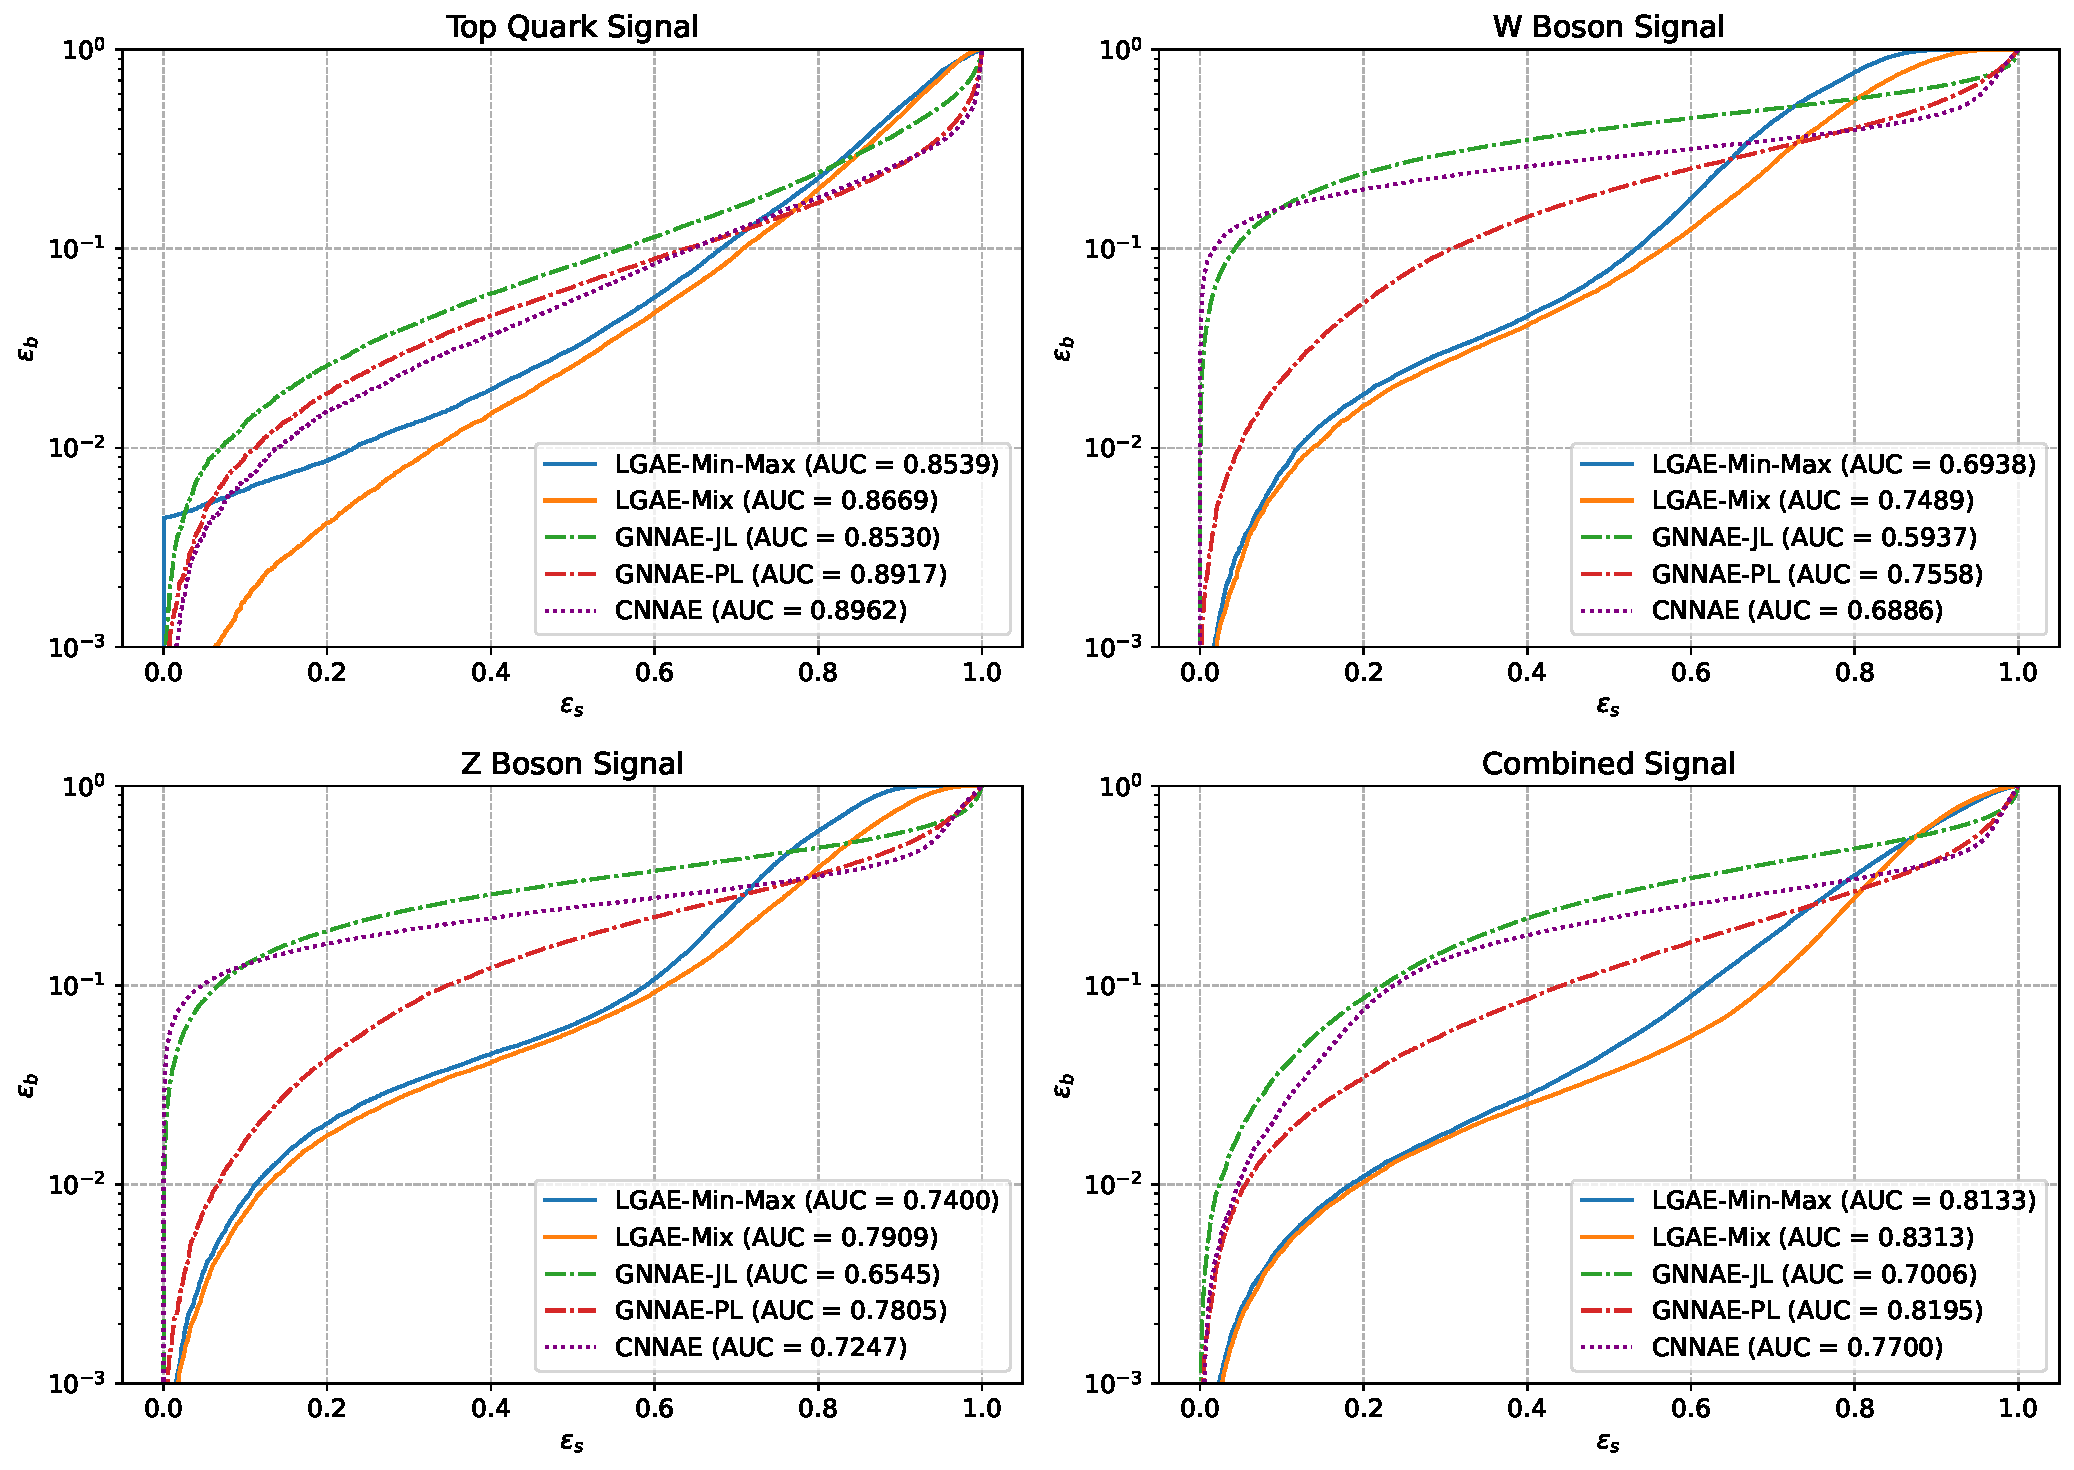
\includegraphics[width=\linewidth]{figures/06-ML4Jets/lgae/anomaly/roc_curves-cnnae.pdf}
    \caption[Anomaly detection ROC curves for the LGAE, GNNAE, and CNNAE models.]{
        Anomaly detection ROC curves for
        the top quark signal (upper left),
        $W$ boson signal (upper right),
        $Z$ boson signal (lower left),
        and the combined signal (lower right)
        by the selected
        LGAE-Min-Max ($\tau_{(1/2, 1/2)} = 7$),
        LGAE-Mix ($\tau_{(1/2, 1/2)}=2$),
        GNNAE-JL ($\dim(L) = 30$),
        GNNAE-PL ($\dim(L) = 2 \times 30$),
        and CNNAE ($\dim(L) = 55$)
        models.
    }
    \label{fig:06_lgae_roc-each}
\end{figure}

We test the performance of all models as unsupervised anomaly detection algorithms by pre-training them solely on QCD and then using the reconstruction error for the QCD and new signal jets as the discriminating variable.
We consider top quark, $\PW$ boson, and $\PZ$ boson jets as potential signals and QCD as the ``background''.
We test the Chamfer distance, energy mover's distance~\cite{Komiske:2019fks} --- the earth mover's distance applied to particle clouds, and MSE between input and output jets as reconstruction errors, and find the Chamfer distance most performant for all graph-based models.
For the CNNAE, we use the MSE between the input and reconstructed image as the anomaly score.

Receiver operating characteristic (ROC) curves showing the signal efficiencies ($\varepsilon_s$) versus background efficiencies ($\varepsilon_b$) for individual and combined signals are shown in Figure~\ref{fig:06_lgae_roc-each},\footnote{Discontinuities in the top quark and combined signal LGAE-Min-Max ROCs indicate that at background efficiencies of $\lessapprox 5\times10^{-3}$, there are no signal events remaining in the validation dataset.} and $\varepsilon_s$ values at particular background efficiencies are given in Table~\ref{tab:06_lgae_ad}.
We see that in general the permutation equivariant LGAE and GNNAE models outperform the CNNAE, strengthening the case for considering equivariance in neural networks.
Furthermore, LGAE models have significantly higher signal efficiencies than GNNAEs and CNNAEs for all signals when rejecting $>90\%$ of the background (which is the minimum level we typically require in HEP), and LGAE-Mix consistently performs better than LGAE-Min-Max.

\begin{table}[ht!]
    \centering
    \caption{
        Anomaly detection metrics by a selected LGAE and GNNAE models, along with the CNNAE model.
        In each column, the best performing latent space per model is italicized, and the best model overall is highlighted in bold.
    }
    \label{tab:06_lgae_ad}
    \resizebox{\textwidth}{!}{
    \begin{tabular}{llllccc } \toprule
        \multirow{2}{*}{Model}       &
        \multirow{2}{*}{Aggregation} & \multirow{2}{*}{Latent space}       & \multirow{2}{*}{AUC}                 &
        \multicolumn{3}{c}{$\varepsilon_s$ at given $\varepsilon_b$}
        \\ \cline{5-7}
        & & & & $\varepsilon_s (10^{-1})$ & $\varepsilon_s (10^{-2})$ & $\varepsilon_s (10^{-3})$ \\ \midrule
        \multirow{6}{*}{LGAE}
        & \multirow{3}{*}{Min-Max}
        & $\tau_{(1/2,1/2)} = 2$ ($30.00\%$)  & $0.7253$ & $0.5706$ & $0.1130$ & $\mathit{0.0011}$                                     \\
                                     &                                     & $\tau_{(1/2,1/2)} = 4$ ($56.67\%$)   & $0.7627$          & $0.5832$                  & $\mathit{0.1305}$         & $0.0007$                  \\
                                     &                                     & $\tau_{(1/2,1/2)} = 7$ ($96.67\%$)   & $\mathit{0.7673}$ & $\mathit{0.5932}$         & $0.0820$                  & $0.0009$                  \\[1mm]
                                     & \multirow{3}{*}{Mix}
                                     & $\tau_{(1/2,1/2)} = 2$ ($15.00\%$)  & $\mathit{0.8023}$                    & $0.6178$          & $\mathbf{0.1662}$         & $\mathbf{0.0250}$                                     \\
                                     &                                     & $\tau_{(1/2,1/2)} = 4$ ($28.33\%$)   & $\mathit{0.8023}$ & $0.6257$                  & $0.1592$                  & $0.0229$                  \\
                                     &                                     & $\tau_{(1/2,1/2)} = 7$ ($48.33\%$)   & $0.7967$          & $\mathbf{0.6290}$         & $0.1562$                  & $0.0225$                  \\[2mm]
        \multirow{5}{*}{GNNAE}
                                     & \multirow{3}{*}{JL}
                                     & $\dim(L) = 10$ ($11.11\%$)          & $0.5891$                             & $0.1576$          & $0.0161$                  & $\mathit{0.0014}$                                     \\
                                     &                                     & $\dim(L) = 40$ ($44.44\%$)           & $0.6636$          & $\mathit{0.2293}$         & $\mathit{0.0262}$         & $0.0013$                  \\
                                     &                                     & $\dim(L) = 80$ ($88.89\%$)           & $\mathit{0.7006}$ & $0.2240$                  & $0.0239$                  & $0.0010$                  \\[1mm]
                                     & \multirow{2}{*}{PL}
                                     & $\dim(L) = 2 \times 30$ ($66.67\%$) & $\mathbf{0.8195}$                    & $\mathit{0.4435}$ & $0.0564$                  & $0.0042$                                              \\
                                     &                                     & $\dim(L) = 3 \times 30$ ($100.00\%$) & $0.8095$          & $0.4306$                  & $\mathit{0.0762}$         & $\mathit{0.0044}$         \\[2mm]
       CNNAE & linear layer
       & $\dim(L) = 55$ ($61.67\%$)
       & $0.7700$
       & $0.2473$
       & $0.0469$
       & $0.0053$ \\
        \cbottomrule
    \end{tabular}
    }
\end{table}


\subsection{Latent space interpretation}
\label{sec:06_lgae_latent-analysis}

\begin{figure}[ht!]
    \centering
    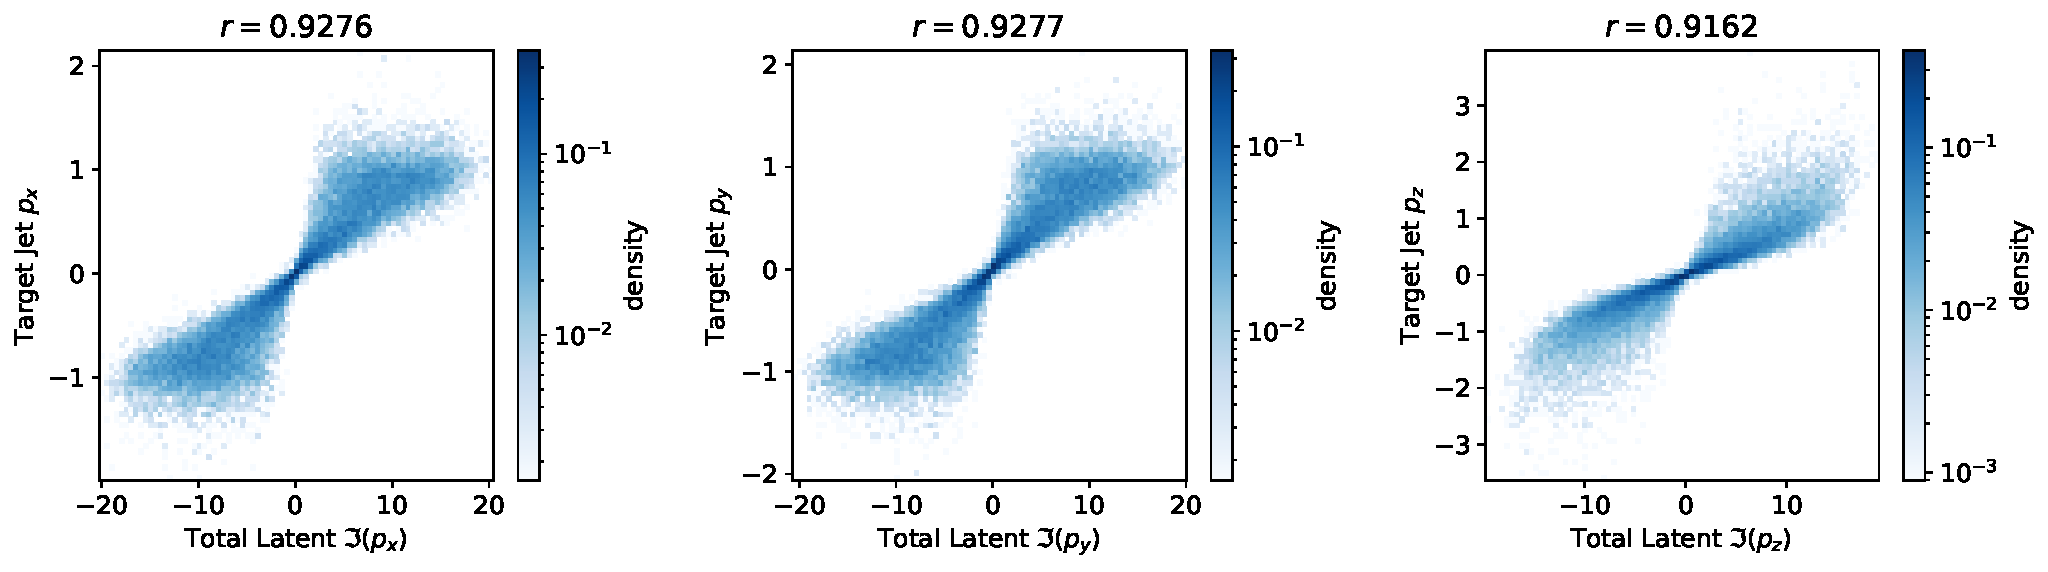
\includegraphics[width=\linewidth]{figures/06-ML4Jets/lgae/latent-space-analysis/corr.pdf}
    \caption{The correlations between the total momentum of the imaginary components in the $\tau_{(1/2, 1/2)} = 2$ LGAE-Mix model and the target jet momenta.
        The Pearson correlation coefficient $r$ is listed above.
    }
    \label{fig:06_lgae_correlations}
\end{figure}

\begin{figure}[ht!]
    \centering
    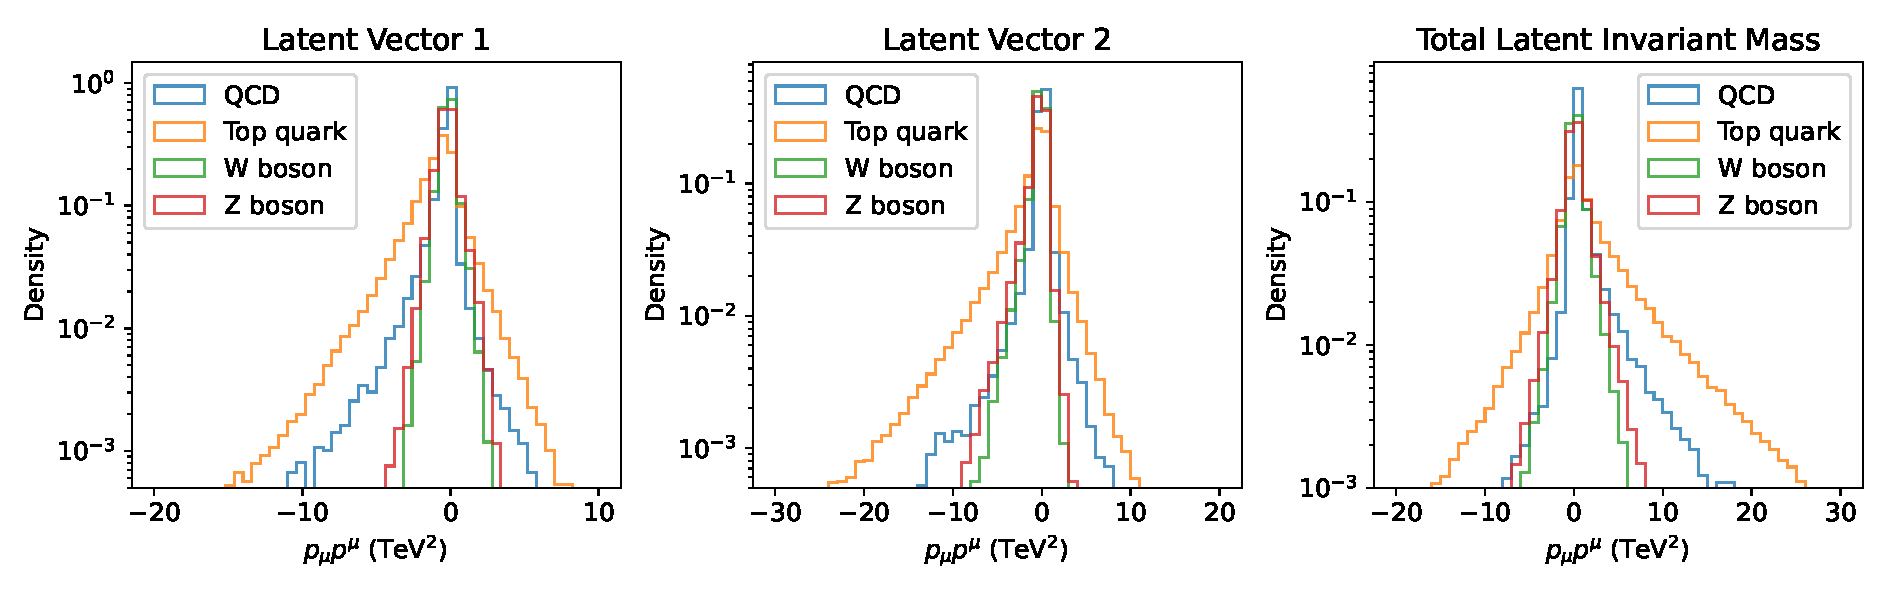
\includegraphics[width=\linewidth]{figures/06-ML4Jets/lgae/latent-space-analysis/invariant_masses-mix-log.pdf}
    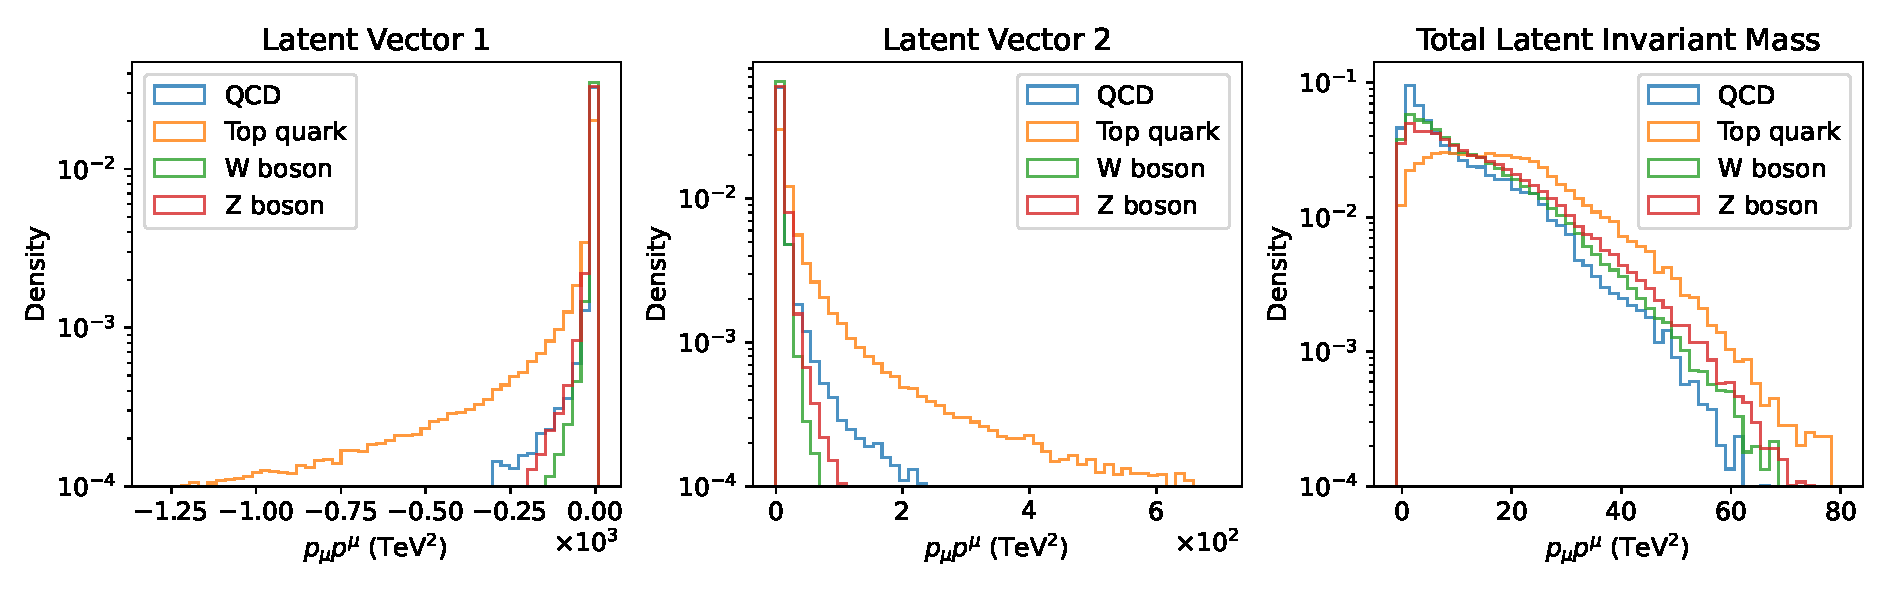
\includegraphics[width=\linewidth]{figures/06-ML4Jets/lgae/latent-space-analysis/invariant_masses-min_max-selected-log.pdf}
    \caption[Distributions of the invariant mass squared of the latent 4-vectors and jet momenta of the LGAE models.]{
        \textbf{Top}: distributions of the invariant mass squared of the latent 4-vectors and jet momenta of the LGAE-Mix with $\tau_{(1/2, 1/2)} = 2$ latent 4-vectors.
        \textbf{Bottom}: distributions of the invariant mass squared of two latent 4-vectors and jet momenta of the LGAE-Min-Max with $\tau_{(1/2, 1/2)} = 2$ latent 4-vectors.
    }
    \label{fig:06_lgae_distribution}
\end{figure}


The outputs of the LGAE encoder are irreducible representations of the Lorentz groups; they consist of a pre-specified number of Lorentz scalars, vectors, and potentially higher-order representations.
This implies a significantly more interpretable latent representation of the jets than traditional autoencoders, as the information distributed across the latent space is now disentangled between the different irreps of the Lorentz group.
For example, scalar quantities like the jet mass will necessarily be encoded in the scalars of the latent space, and jet and particle 4-momenta in the vectors.

We demonstrate the latter empirically on the LGAE-Mix model ($\tau_{(1/2, 1/2)} = 2$) by looking at correlations between jet 4-momenta and the components of different combinations of latent vector components.
Figure~\ref{fig:06_lgae_correlations} shows that, in fact, the jet momenta is encoded in the imaginary component of the sum of the latent vectors.

We can also attempt to understand the anomaly detection performance by looking at the encodings of the training data compared to the anomalous signal.
Figure~\ref{fig:06_lgae_distribution} shows the individual and total invariant mass of the latent vectors of sample LGAE models for QCD and top quark, W boson, and Z boson inputs.
We observe that despite the overall similar kinematic properties of the different jet classes, the distributions for the QCD background are significantly different from the signals, indicating that the LGAE learns and encodes the difference in jet substructure --- despite substructure observables such as jet mass not being direct inputs to the network --- explaining the high performance in anomaly detection.

Finally, while in this section we showcased simple ``brute-force'' techniques for interpretability by looking directly at the distributions and correlations of latent features, we hypothesize that such an equivariant latent space would also lend itself effectively to the vast array of existing explainable AI algorithms~\cite{vilone_xaireview,minh_xaireview}, which generically evaluate the contribution of different input and intermediate neuron features to network outputs.
We leave a detailed study of this to future work.


\subsection{Data efficiency}
\label{sec:06_lgae_data-efficiency}

\begin{figure}[ht!]
    \centering
    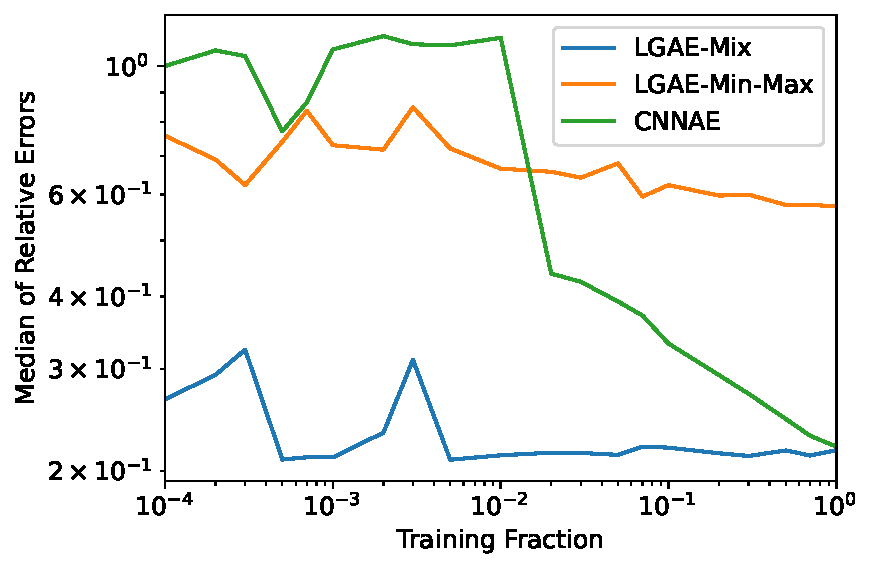
\includegraphics[width=0.6\linewidth]{figures/06-ML4Jets/lgae/data_efficiency/jet_mass-rel_err-median.pdf}
    \caption{Median magnitude of relative errors of jet mass reconstruction by LGAE and CNNAE models at trained on different fractions of the training data.}
    \label{fig:06_lgae_median-jet-mass}
\end{figure}

In principle, equivariant neural networks should require less training data for high performance, since critical biases of the data, which would otherwise have to be learned by non-equivariant networks, are already built in.
We test this claim by measuring the performances of the best-performing LGAE and CNNAE architectures from Section~\ref{sec:06_lgae_reconstruction} trained on varying fractions of the training data.

The median magnitude of the relative errors between the reconstructed and true jet masses of the different models and fractions is shown in Figure~\ref{fig:06_lgae_median-jet-mass}.
Each model is trained five times per training fraction, with different random seeds, and evaluated on the same-sized validation dataset; the median of the five models is plotted.
We observe that, in agreement with our hypothesis, the LGAE models both maintain their high performance all the way down to training on 1\% of the data, while the CNNAE's performance steadily degrades down to 2\% and then experiences a further sharp drop.


\section{Conclusion}
\label{sec:06_lgae_conclusion}

We develop the Lorentz group autoencoder (LGAE), an autoencoder model equivariant to Lorentz transformations.
We argue that incorporating this key inductive bias of high energy physics (HEP) data can have a significant impact on the performance, efficiency, and interpretability of machine learning models in HEP.
We apply the LGAE to tasks of compression and reconstruction of input quantum chromodynamics (QCD) jets, and of identifying anomalous top quark, W boson, and Z boson jets.
We report excellent performance in comparison to baseline graph and convolutional neural network autoencoder models, with the LGAE outperforming them on several key metrics.
We also demonstrate the LGAE's interpretability, by analyzing the latent spaces of LGAE models for both tasks, and data efficiency relative to baseline models.
The LGAE opens many promising avenues in terms of both performance and model interpretability, with the exploration of new datasets, the magnitude of Lorentz and permutation symmetry breaking due to detector effects, higher-order Lorentz group representations, and challenges with real-life compression and anomaly detection applications all exciting possibilities for future work.

\subsubsection{Acknowledgements}

This chapter is, in part, a reprint of the materials as they appear in
Eur. Phys. J. C, 2023, Z. Hao; R. Kansal; J. Duarte; and N. Chernyavskaya; Lorentz group equivariant autoencoders.
The dissertation author was the primary investigator and (co-)author of this paper.
